\documentclass[
    a4paper,
    12pt,
    english,
    brazilian
]{article}

% --- Codificação/Fontes p/ pdflatex ---
\usepackage[utf8]{inputenc}
\usepackage[T1]{fontenc}

\PassOptionsToPackage{hidelinks,unicode}{hyperref}
\PassOptionsToPackage{nameinlink,noabbrev}{cleveref}

% --- Pacotes necessários ---
\usepackage[hidelinks,unicode]{hyperref}
\usepackage{graphicx}   % para \includegraphics
\usepackage[]{fatec-article}
\usepackage{float}
\usepackage{array}
\usepackage{longtable}
\usepackage{setspace}
\usepackage{multirow}
\usepackage{tocloft}

\usepackage[utf8]{inputenc}
\usepackage{array}
\usepackage{geometry}
\usepackage{adjustbox}
\usepackage{caption}
\usepackage{tabularx}
\usepackage{ragged2e}
\usepackage{caption}
\usepackage{adjustbox}
\usepackage{booktabs}
\usepackage{longtable} 
\usepackage{float}
\usepackage{placeins}

\geometry{top=1.5cm, bottom=1.5cm, left=1.2cm, right=1.2cm}

% --- Cabeçalho FATEC com controles de espaçamento ---
% Ajustes fáceis:
\newcommand{\LogoWidth}{0.23\textwidth}   % largura do bloco da logo
\newcommand{\LogoHeight}{4.5cm}           % altura da logo
\newcommand{\HeaderGutter}{1em}           % espaço entre logo e textos
\newcommand{\HeaderTightness}{-2.3\baselineskip} % <- aproxima a LINHA do texto (mais negativo = mais perto)

\newcommand{\fatecCabecalho}{%
    \noindent
    \begin{minipage}[c]{\LogoWidth}
        
\includegraphics[height=\LogoHeight]{Images/fatec.jpg}%
    \end{minipage}\hspace*{\HeaderGutter}%
    \begin{minipage}[c]{\dimexpr\textwidth-\LogoWidth-\HeaderGutter\relax}
        \raggedright\small
        Governo do Estado de São Paulo\\
        \textbf{Faculdade de Tecnologia do Estado de São Paulo}\\
        Centro Estadual de Educação Tecnológica Paula Souza\\
        Desenvolvimento de Software Multiplataforma
    \end{minipage}

    % Esta linha controla o quão perto a régua fica do texto:
    \vspace*{\HeaderTightness}%
    \noindent\rule{\textwidth}{0.5pt}
}

% --- CONFIG DO SUMÁRIO (estilo da imagem) ---
\renewcommand{\contentsname}{Sumário}
\setcounter{tocdepth}{2}                 % mostra até subseção
\renewcommand{\cftsecaftersnum}{.}       % "1."
\renewcommand{\cftsubsecaftersnum}{.}    % "1.1."
\renewcommand{\cftsecleader}{\cftdotfill{\cftdotsep}}
\renewcommand{\cftsubsecleader}{\cftdotfill{\cftdotsep}}
\setlength{\cftsecnumwidth}{3em}
\setlength{\cftsubsecnumwidth}{4em}
% (não usamos \cftsecfont=\MakeUppercase aqui para evitar erro)

% --- Título e autores no preâmbulo ---
\title{ARTEFATOS DO PROJETO DE SOFTWARE\\[0.7em]
CLASSIFICAÇÃO DE MANGANÊS E COBRE NA FOLHA DA MEXERICA,\\
ORIENTADO POR REDES NEURAIS}
\author{%
A. Freitas \texttt{\{ amanda.freitas14@fatec.sp.gov.br \}}\\
L. Fagundes \texttt{\{ lucas.fagundes3@fatec.sp.gov.br \}}\\
V. Freitas \texttt{\{ valeria.freitas@fatec.sp.gov.br \}}
}

% --- Início do Documento ---
\begin{document}

\vspace{-5cm}
\fatecCabecalho
\vspace{8cm}
\begin{center}
    \large \textbf{\title{ARTEFATOS DO PROJETO DE SOFTWARE}}\\[1em]
    \large \textbf{\title{CLASSIFICAÇÃO DE MANGANÊS E COBRE NA FOLHA DA MEXERICA, ORIENTADO POR REDES NEURAIS}}\\[1.2em]

    \normalsize
    Freitas. A \textbf{\{ amanda.freitas14@fatec.sp.gov.br \}}\\
    Fagundes. L \textbf{\{ lucas.fagundes3@fatec.sp.gov.br \}}\\
    Freitas. V \textbf{\{ valeria.freitas@fatec.sp.gov.br \}}

\end{center}


\clearpage
\tableofcontents
\clearpage

% ------------------------------------------------------------------
% Seções
% ------------------------------------------------------------------

% --- Diagramas UML ---
\section[\MakeUppercase{Diagramas UML}]{Diagramas UML}
Nesta seção serão apresentados os diagramas da UML utilizados para a modelagem do sistema desenvolvido. Dentre
os diagramas utilizados, pode-se citar: Diagrama de Caso de Uso, Diagrama de Classe e Diagrama de Objetos.

% ------------------------------------------------------------------
    \subsection{\textbf{Diagrama de Caso de Uso}}
    \label{sect:Casos-de-uso}
    \noindent\textbf{Atores do Sistema:}
\begin{itemize}[itemsep=0.6em, topsep=0.3em, parsep=0pt]
    \item \textbf{Usuário (Cliente)}: acessa o sistema para realizar cadastro/login, consultar informações, criar/editar solicitações e acompanhar status.
    \item \textbf{Administrador}: gerencia cadastros, permissões, configurações gerais e monitora registros/relatórios.
    \item \textbf{Operador/Atendente}: valida dados enviados pelos usuários, aprova/reprova solicitações e atualiza status operacionais.
    \item \textbf{Sistema Externo (API/Integrações)}: provê/autentica dados de serviços de terceiros (ex.: pagamento, mapas, notificações).
\end{itemize}

\vspace{0.9\baselineskip}

\noindent\textbf{Casos de Uso do Sistema:}
\begin{itemize}[itemsep=0.6em, topsep=0.3em, parsep=0pt]
    \item \textbf{Autenticar Usuário}: realizar cadastro, login e recuperação de senha.
    \item \textbf{Gerenciar Perfis}: editar dados pessoais, preferências e documentos.
    \item \textbf{Registrar Solicitação}: criar, editar e cancelar solicitações (com validações e anexos).
    \item \textbf{Acompanhar Status}: visualizar andamento, receber notificações e histórico.
    \item \textbf{Gerir Operações (Backoffice)}: triagem, aprovação/reprovação e ajustes operacionais.
    \item \textbf{Relatórios e Auditoria}: visualizar métricas, exportar dados e rastrear logs.
    \item \textbf{Integrações}: consultar/enviar dados para APIs externas (pagamentos, geolocalização, e-mail/SMS).
\end{itemize}

\begin{figure}[H]
\centering
\caption{Diagrama de caso de uso}
\label{fig:diagrama-caso-uso}
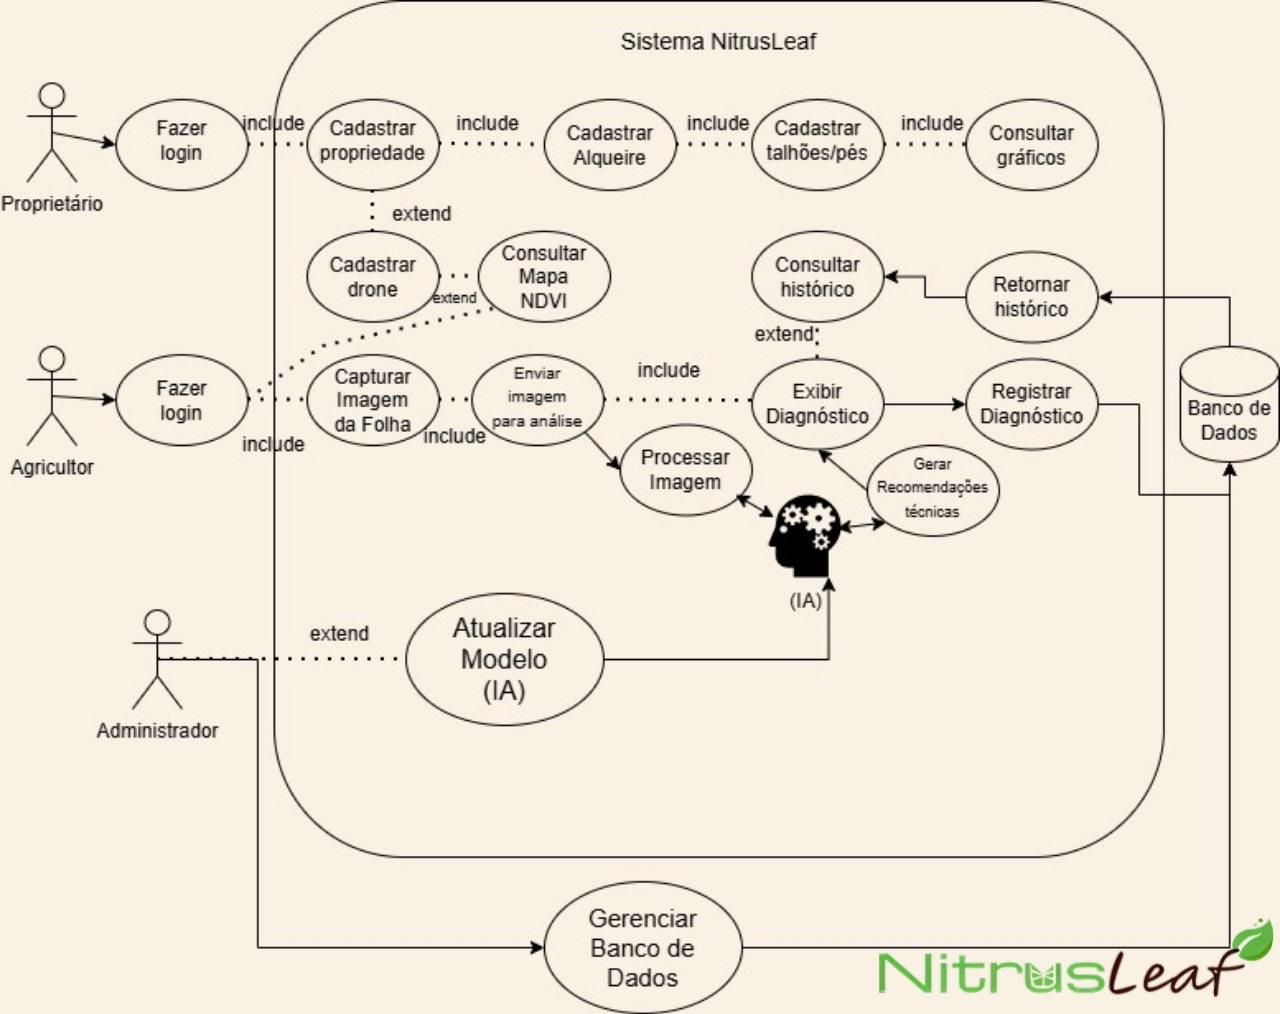
\includegraphics[width=0.8\textwidth]{Images/DiagramaCasosDeUso.jpg}
\SourceOrNote{Equipe 21 - Vitalliz (2025)}
\end{figure}

O diagrama acima ilustra as principais interações entre os usuários e o sistema,
evidenciando os processos relacionados ao monitoramento de deficiências nutricionais
em plantações de mexerica com o apoio de tecnologia de drones.
\medskip

% ------------------------------------------------------------------
    \subsection{\textbf{Diagrama de Classe}}
    \label{sect:Diagrama-de-classe}
    O diagrama da Figura 2 resume um sistema de gestão agrícola com classes para Usuário, Propriedade, Talhão e 
Diagnóstico, além de ServidorNode, ProcessamentoPython, BancoDeDados e PainelAdmin. Juntas, elas cobrem do 
login e cadastro ao registro de áreas, classificação de imagens por CNN e armazenamento/gestão dos resultados.

\medskip
\noindent{As principais classes e seus papéis são:}
\begin{itemize}[itemsep=0.6em, topsep=0.3em, parsep=0pt]
    \item \textbf{Propriedade}: Cadastra e gerencia propriedades rurais (endereço completo, cidade, CEP), vinculadas a um idUsuario; permite criar/editar e listar talhões da propriedade.
    \item \textbf{Usuario}: Mantém dados pessoais e de autenticação (nome, e-mail, telefone, senha, tipo); oferece cadastro, edição de perfil e login para controle de acesso.
    \item \textbf{Talhao}: Subárea da propriedade. Guarda id e nome, ligado a uma Propriedade. Permite cadastrar/editar e consultar o histórico de diagnósticos do local.
    \item \textbf{Diagnostico}: Registro de análise por imagem de folha. Liga-se a um Talhão e salva data, resultado e probabilidade. Métodos: enviar imagem, receber e visualizar resultado.
    \item \textbf{ServidorNode}: Faz a ponte do frontend com a API; recebe requisições, encaminha para o módulo Python, monitora status e salva resultados no banco.
    \item \textbf{ProcessamentoPython}: Executa classificação de imagens com CNN, controla versões dos modelos e permite atualizar/rodar modelos para análise agrícola.
    \item \textbf{BancoDeDados}: Gerencia a conexão e as operações CRUD; insere, consulta e atualiza registros, sustentando a persistência de todo o sistema.
    \item \textbf{PainelAdmin}: Área do administrador para gestão global; visualiza usuários, monitora o sistema e atualiza modelos de CNN, garantindo o controle da plataforma.
\end{itemize}

\begin{figure}[H]
\centering
\caption{Diagrama de classe}%
\label{fig:diagrama-classe}
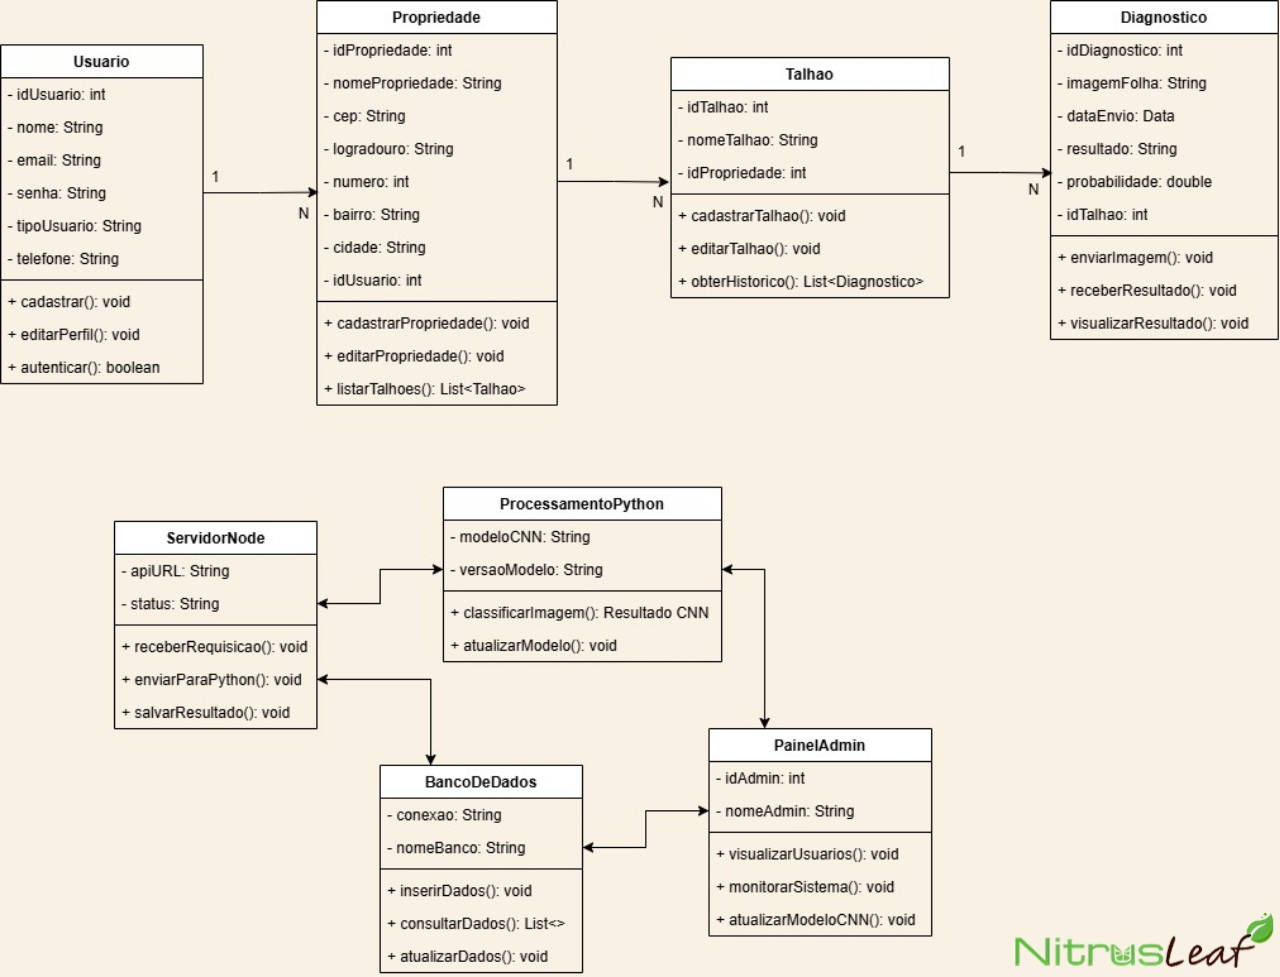
\includegraphics[width=0.8\textwidth]{Images/DiagramaDeClasses.jpg}
\SourceOrNote{Equipe 21 - Vitalliz (2025)}
\end{figure}

O diagrama mostra claramente os relacionamentos de composição e agregação
entre as entidades, com cardinalidades bem definidas. Além disso, os métodos estão
especificados em várias classes, indicando a lógica operacional do sistema, e a
estrutura geral está organizada para refletir um fluxo de uso coerente com os casos de
uso anteriores.
\medskip

% ---------------------------------------------------------- --------
    \subsection{\textbf{Diagrama de Objetos}}
    \label{sect:Diagrama-de-objetos}
    O diagrama de objetos a seguir exemplifica, com instâncias concretas, partes do sistema previamente modelado:
são criados objetos de CadastrarDadosUsuario (abrangendo usuários dos tipos físico e jurídico), 
CadastrarDadosPropriedade e CadastrarTalhão, evidenciando o fluxo de criação e vinculação entre eles. Assim, 
o exemplo mostra como um usuário é instanciado com seus atributos, em seguida uma propriedade é cadastrada e 
associada a esse usuário, e por fim um talhão é criado e ligado à propriedade, ilustrando de forma prática 
as relações e o ciclo de cadastro definidos no diagrama de classes.

\begin{figure}[H]
\centering
\caption{Diagrama de objetos}%
\label{fig:diagrama-objetos}
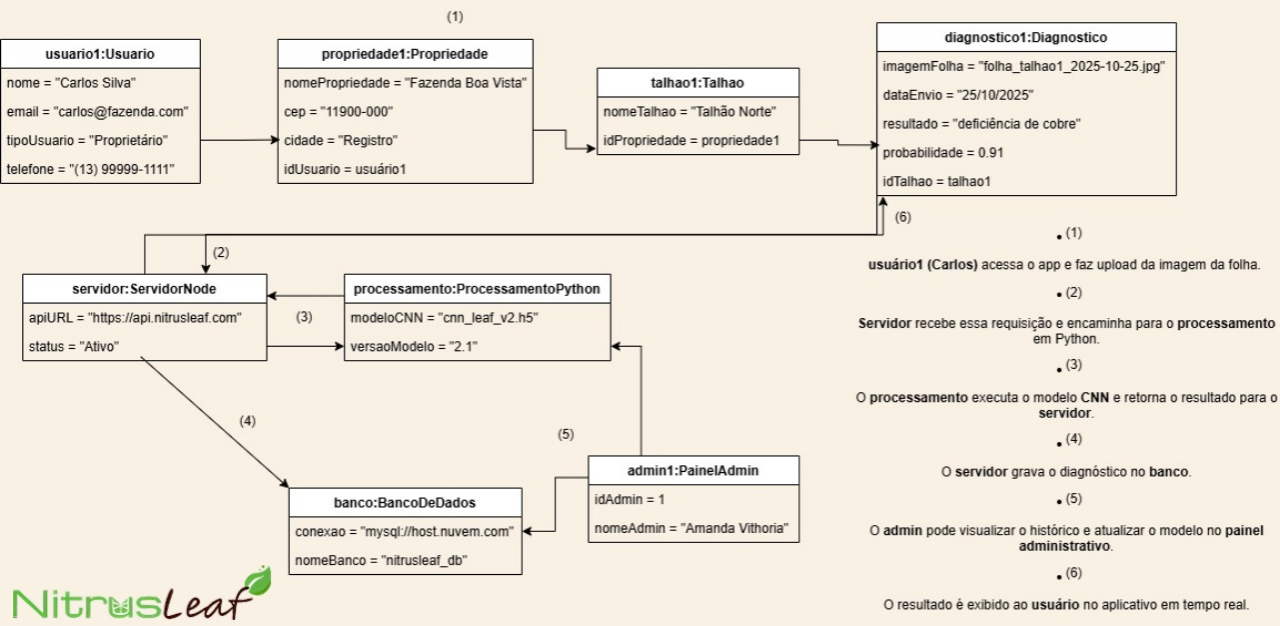
\includegraphics[width=0.8\textwidth]{Images/DiagramaDeObjetos.jpg}
\SourceOrNote{Equipe 21 - Vitalliz (2025)}
\end{figure}

O diagrama usa valores realistas (nomes, CEP, cidade, URLs) e encadeia o fluxo completo
do upload da folha pelo produtor até o diagnóstico gravado e exibido, com supervisão do admin
e versionamento do modelo.
\medskip

% ------------------------------------------------------------------

% --- Diagramas de Banco de Dados ---
\section{Diagramas de Banco de Dados}{Diagramas de Banco de Dados}
A seguir são apresentados os diagramas de banco de dados que ilustram a
estrutura e os relacionamentos das tabelas utilizadas no sistema.

% ------------------------------------------------------------------
    \subsection{\textbf{Diagrama Entidade-Relacionamento (DER)}}
    \label{sect:Diagrama-Entidade-Relacionamento}
    
\medskip
O diagrama a seguir representa o Modelo Entidade–Relacionamento (DER) do sistema \textit{Nitrusleaf}, 
descrevendo a estrutura lógica do banco de dados. As entidades, seus atributos e os relacionamentos 
foram definidos conforme os requisitos do sistema, assegurando integridade e suporte às funcionalidades 
de operação e análise.

\medskip
A entidade \textbf{Usuários} centraliza as informações de acesso e cadastro 
(incluindo \textit{tipo\_pessoa}, foto, CPF/CNPJ e dados de contato/endereço). Ela se relaciona 
com \textbf{Propriedades} pelo relacionamento \textbf{Possui}: um usuário pode não possuir ou 
possuir várias propriedades (0:N) e cada propriedade pertence a um único usuário (1:1).
\medskip

As \textbf{Propriedades} armazenam dados cadastrais (logradouro, CEP, cidade) e contadores globais 
(\textit{talhoes\_registrados}, \textit{total\_pes}). Cada propriedade \textbf{contém} múltiplos 
\textbf{Talhões} (1:N) e também \textbf{contém} diversos \textbf{Alqueires} (1:N). Os \textbf{Talhões} 
registram metadados produtivos (espécie/fruta, \textit{total\_pes}, \textit{pes\_analisados}, 
\textit{pes\_diagnosticados}).
\medskip

Dentro de cada talhão são cadastrados os \textbf{Pés} (plantas individuais), em relacionamento 1:N 
(Talhão~$\rightarrow$~Pés). A entidade \textbf{Pés} guarda a situação atual e campos de diagnóstico 
(\textit{deficiencia\_cobre}, \textit{deficiencia\_manganes}, \textit{outros}, \textit{observacoes}).
\medskip

O histórico temporal de cada planta é mantido por \textbf{Historico\_pe}, ligado a \textbf{Pés} pelo 
relacionamento \textbf{Armazena}: um pé pode possuir muitos registros (descrição, \textit{data\_criacao}, 
situação) e cada registro referencia um único pé (e seu talhão no momento do evento).
\medskip

As avaliações visuais são registradas em \textbf{Fotos}. Pelo relacionamento \textbf{Analisado\_por}, 
um Pé pode ter muitas fotos (1:N) e cada Foto está vinculada a um único pé (URL, \textit{data\_tiragem}, 
\textit{resultado\_analise}).
\medskip

A partir das fotos, o sistema gera \textbf{Relatórios}. Cada Relatório é produzido a partir de uma 
única Foto e vincula-se a um único Pé, consolidando \textit{data da análise}, achados de deficiência 
(cobre, manganês, outros) e observações. O relacionamento \textbf{Tem\_relatorios} expressa que um pé 
pode possuir vários relatórios (1:N), e \textbf{Gera} indica a origem do relatório a partir de uma foto 
(uma foto pode originar relatórios reprocessados).
\medskip

\begin{figure}[H]
\centering
\caption{Diagrama Entidade–Relacionamento}
\label{fig:diagrama-der}
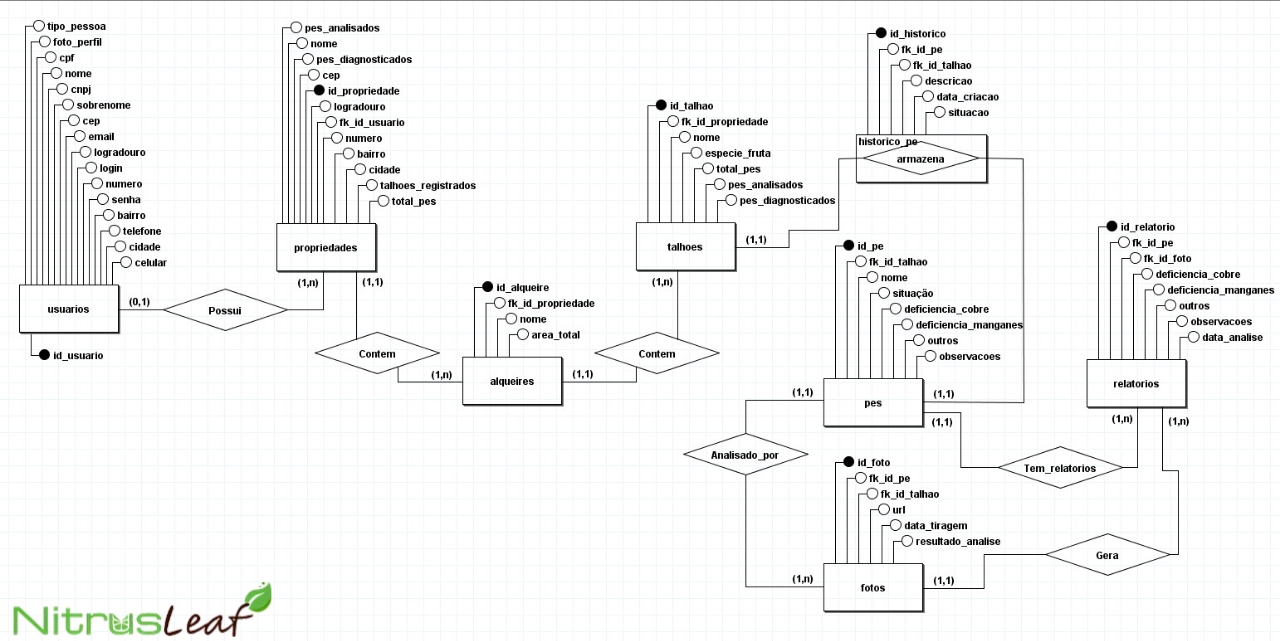
\includegraphics[width=0.9\textwidth]{Images/DiagramaDER.jpg}
\SourceOrNote{Equipe 21 -- Vitalliz (2025)}
\end{figure}

Esse modelo é fundamental para garantir a integridade dos dados e a correta
estruturação das informações no sistema.
\medskip

% ------------------------------------------------------------------
    \subsection{\textbf{Diagrama Modelo Lógico (MER)}}
    \label{sect:Diagrama-Modelo-Lógico}
    \input{Topicos/Diagrama-Modelo-Lógico}


% --- Canvas ---
\section{Modelo de Negócios Canvas}
A seguir são apresentados os diagramas de banco de dados que ilustram a
estrutura e os relacionamentos das tabelas utilizadas no sistema.

\label{sect:Canvas}
\medskip
\noindent\textbf{Proposta de Valor}\\
O sistema tem como objetivo central ajudar os agricultores a identificarem deficiências de manganês e cobre nas folhas de mexerica, contribuindo para manter o padrão de qualidade da fruta. A utilização de inteligência artificial integrada ao sistema oferece precisão na análise das fotos enviadas pelos usuários.

\medskip
\noindent\textbf{Segmento de Mercado}\\
O público-alvo são os agricultores de mexerica do Vale do Ribeira, com foco específico em produtores rurais, horticultores e demais interessados na melhoria da produtividade agrícola.

\medskip
\noindent\textbf{Relacionamento com o Cliente}\\
O relacionamento com os usuários será realizado via WhatsApp, aplicativo móvel e site institucional. Os usuários poderão enviar fotos das folhas e receber feedback automatizado por meio de gráficos e mapas gerados pelo sistema. O aplicativo também permite o envio de análises e resultados personalizados.

\medskip
\noindent\textbf{Canais}\\
A divulgação e o acesso ao sistema ocorrerão por meio de anúncios em secretarias de agricultura dos municípios da região, com suporte adicional via site, e-mail e WhatsApp da empresa, fortalecendo a comunicação direta com o público-alvo.

\medskip
\noindent\textbf{Atividades-Chave}\\
As principais atividades envolvem a identificação de deficiência nutricional nas folhas e o fornecimento de suporte técnico e manutenção contínua do sistema.

\medskip
\noindent\textbf{Recursos-Chave}\\
Para operar corretamente, o sistema depende de uma equipe técnica composta por programadores, instaladores do sistema físico e profissionais responsáveis pelo suporte online. Além disso, é necessário um serviço de hospedagem para o site e para o banco de dados.

\medskip
\noindent\textbf{Parcerias-Chave}\\
As parcerias incluem associações de fazendeiros, secretarias de agricultura locais e participação em feiras do setor agrícola, que auxiliam na disseminação e na credibilidade do projeto.

\medskip
\noindent\textbf{Estrutura de Custos}\\
Inclui gastos com manutenção dos equipamentos de monitoramento, aluguel de espaço físico para atendimento, aquisição de materiais e tecnologias para análise das folhas, além de custos com servidores para armazenamento dos dados.

\medskip
\noindent\textbf{Fontes de Renda}\\
A monetização ocorre por meio do aluguel do sistema, da cobrança pelo aluguel de equipamentos necessários e da prestação de serviços de instalação e manutenção.
\medskip

\begin{figure}[H]
\centering
\caption{Modelo de Negócios Canvas}
\label{fig:Canvas}
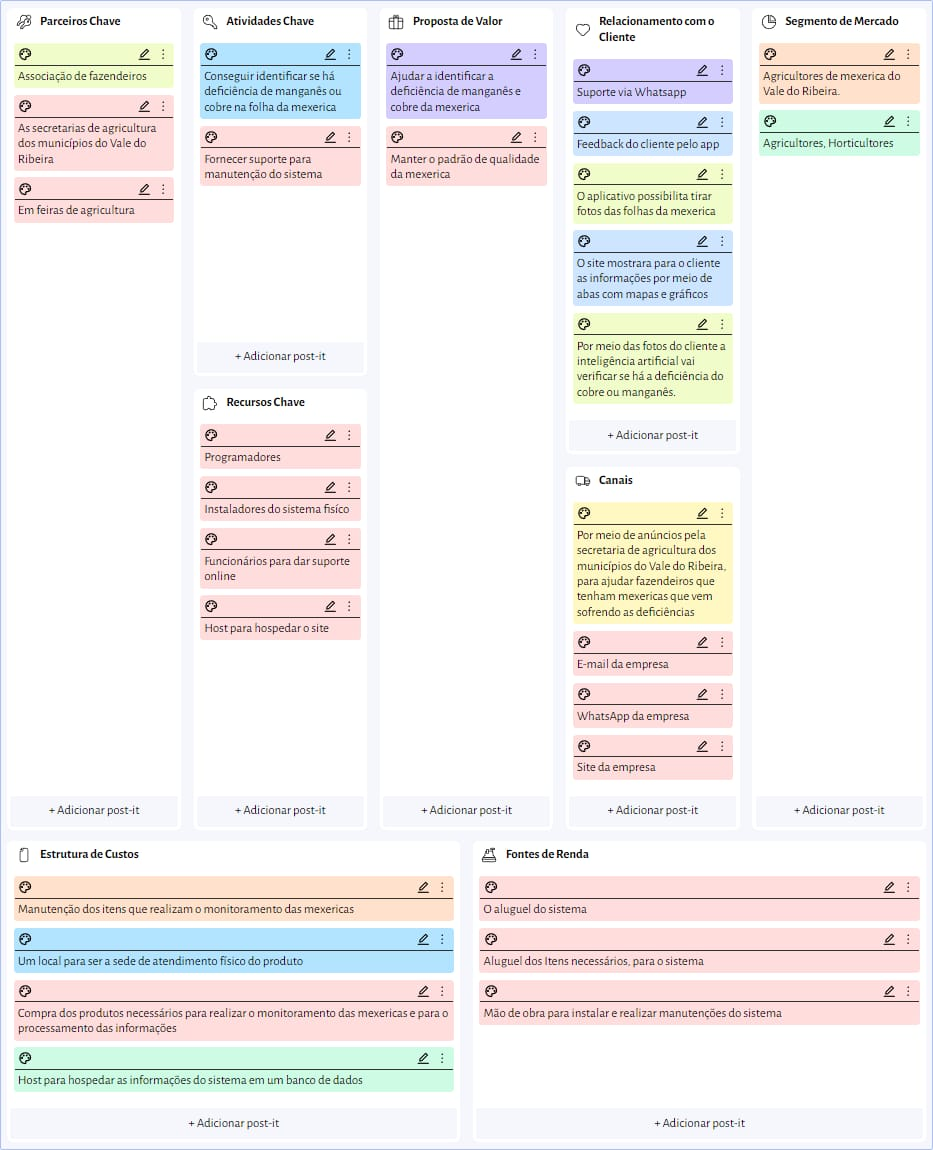
\includegraphics[width=0.8\textwidth]{Images/Canvas.jpeg}
\SourceOrNote{Equipe 21 - Vitalliz (2025)}
\end{figure}
\medskip


% --- Diagramas de Redes ---
\section{DIAGRAMA E ESPECIFICAÇÕES DA INFRAESTRUTURA DE REDE}
Esta seção descreve a estrutura lógica e física da rede interna utilizada para o
funcionamento do sistema de monitoramento e análise de folhas de mexerica,
conforme representado no diagrama a seguir.

% ------------------------------------------------------------------
    \subsection{\textbf{Visão Geral da Rede}}
    \label{sect:Visao-geral-da-Rede}
    

A infraestrutura NitrusLeaf centraliza o diagnóstico agrícola, onde o Agricultor envia imagens de 
plantas via internet (HTTPS) para o Servidor da Sede, que as processa usando Inteligência Artificial 
(IA) para identificar problemas. Os resultados são armazenados em um Banco de Dados na Nuvem e 
o servidor devolve ao usuário um diagnóstico e uma recomendação prática. O sistema é mantido e aprimorado
por um Administrador que atualiza os modelos de IA, garantindo a segurança dos dados e a precisão das 
análises de campo

% ------------------------------------------------------------------
    \subsection{\textbf{Componentes da Rede}}
    \label{sect:Componentes-da-Rede}
    \noindent\textbf{Nuvem (Servidor Externo:)}\par
Hospeda os serviços centrais do sistema: \textit{API Node.js} (ponto de entrada das requisições), 
\textit{Banco MySQL} (armazenamento de propriedades, diagnósticos, imagens e histórico) e 
\textit{Processamento de Imagens (IA)} (análises e geração de resultados). A comunicação externa 
ocorre via \textbf{HTTPS/TLS}, enquanto a comunicação interna entre serviços permanece em sub-redes 
privadas com regras de segurança (grupos de segurança/firewall). Proporciona \textit{escala}, 
\textit{alta disponibilidade} e \textit{monitoramento/logs} para auditoria e desempenho.

\medskip
\noindent\textbf{Roteador (Acesso do Cliente:)}\par
Responsável por interligar a \textbf{rede local da propriedade} à internet (fibra/rádio/4G--5G). 
Encaminha o tráfego \textbf{HTTPS} dos dispositivos dos usuários até a API na nuvem e recebe as respostas
(diagnóstico e recomendações). Executa \textit{NAT}, pode fornecer \textit{DHCP} e aplicar \textit{QoS} 
para priorizar upload de imagens. Opcionalmente estabelece \textit{VPN} para gestão remota segura e 
implementa políticas básicas de firewall na borda do cliente.

\medskip
\noindent\textbf{Rede (LAN \& WAN:)}\par
A \textbf{LAN da Propriedade} conecta os endpoints (PC do Proprietário e smartphone do Agricultor) 
por cabo/wi-fi, podendo usar \textit{switch} para segmentação e ampliação de portas. A 
\textbf{WAN (Internet/Nuvem)} é o meio público IP que transporta os dados entre cliente e serviços 
em nuvem com \textbf{TLS} de ponta a ponta. Fluxo típico: \textit{Dispositivo} $\rightarrow$ 
\textit{Roteador (LAN)} $\rightarrow$ \textit{Internet (WAN)} $\rightarrow$ 
\textit{API Node.js (Nuvem)} $\rightarrow$ \textit{MySQL/IA (Nuvem)} $\rightarrow$ 
\textit{Resposta ao usuário}.
\medskip

% ------------------------------------------------------------------
    \subsection{\textbf{Fluxo de Comunicação}}
    \label{sect:Fluxo-de-comunicacao}
    \noindent\textbf{Internamente (Rede)}
\begin{itemize}
    \setlength{\itemsep}{0.8em}   % espaço entre itens
    \setlength{\topsep}{0.4em}    % espaço antes/depois da lista
    \setlength{\parsep}{0pt}      % espaço entre parágrafos dentro do item
    \setlength{\parskip}{0pt}
    \item \textbf{Switch}: interliga os computadores dos setores (desenvolvimento, manutenção e recepção) na LAN, comutando o tráfego local.
    \item \textbf{Roteador (NAT/Firewall)}: conecta a LAN à Internet, aplica NAT e regras de firewall, garantindo que os hosts internos acessem serviços externos com segurança.
    \item \textbf{Saída para a Internet}: provê conectividade externa para o acesso ao site/app e para a comunicação com a API.
\end{itemize}

\medskip
\noindent\textbf{Externamente (Cliente \(\leftrightarrow\) Sede via Internet)}
\begin{itemize}
    \setlength{\itemsep}{0.8em}
    \setlength{\topsep}{0.4em}
    \setlength{\parsep}{0pt}
    \setlength{\parskip}{0pt}
    \item \textbf{Canal}: comunicação realizada via \textbf{HTTPS} sobre a Internet pública.
    \item \textbf{Fluxo de alto nível}: o cliente envia imagens \(\rightarrow\) o tráfego chega à \textbf{API (Servidor Node.js)} \(\rightarrow\) a API orquestra processamento/armazenamento \(\rightarrow\) o diagnóstico é retornado ao cliente (site/app).
    \item \textbf{Observações de rede}: o cliente \textbf{não acessa diretamente} o módulo de IA nem o banco; a LAN permanece isolada atrás do NAT do roteador.
\end{itemize}
\medskip

% ------------------------------------------------------------------
    \subsection{\textbf{Segurança e Estabilidade}}
    \label{sect:Seguranca-e-estabilidade}
    \medskip
\noindent{Para garantir a estabilidade da comunicação e a segurança dos dados:}
\begin{itemize}
    \item Utiliza-se autenticação segura no acesso ao sistema;.
    \item O tráfego de informações entre o usuário e o servidor é criptografado;
    \item O roteador é configurado com firewall e controle de acesso;
    \item O servidor é mantido em ambiente cloud com redundância e backups regulares.
\end{itemize}

\medskip

\begin{figure}[H]
\centering
\caption{Diagrama Infraestrutura de Redes}
\label{fig:diagrama-infraestrutura}
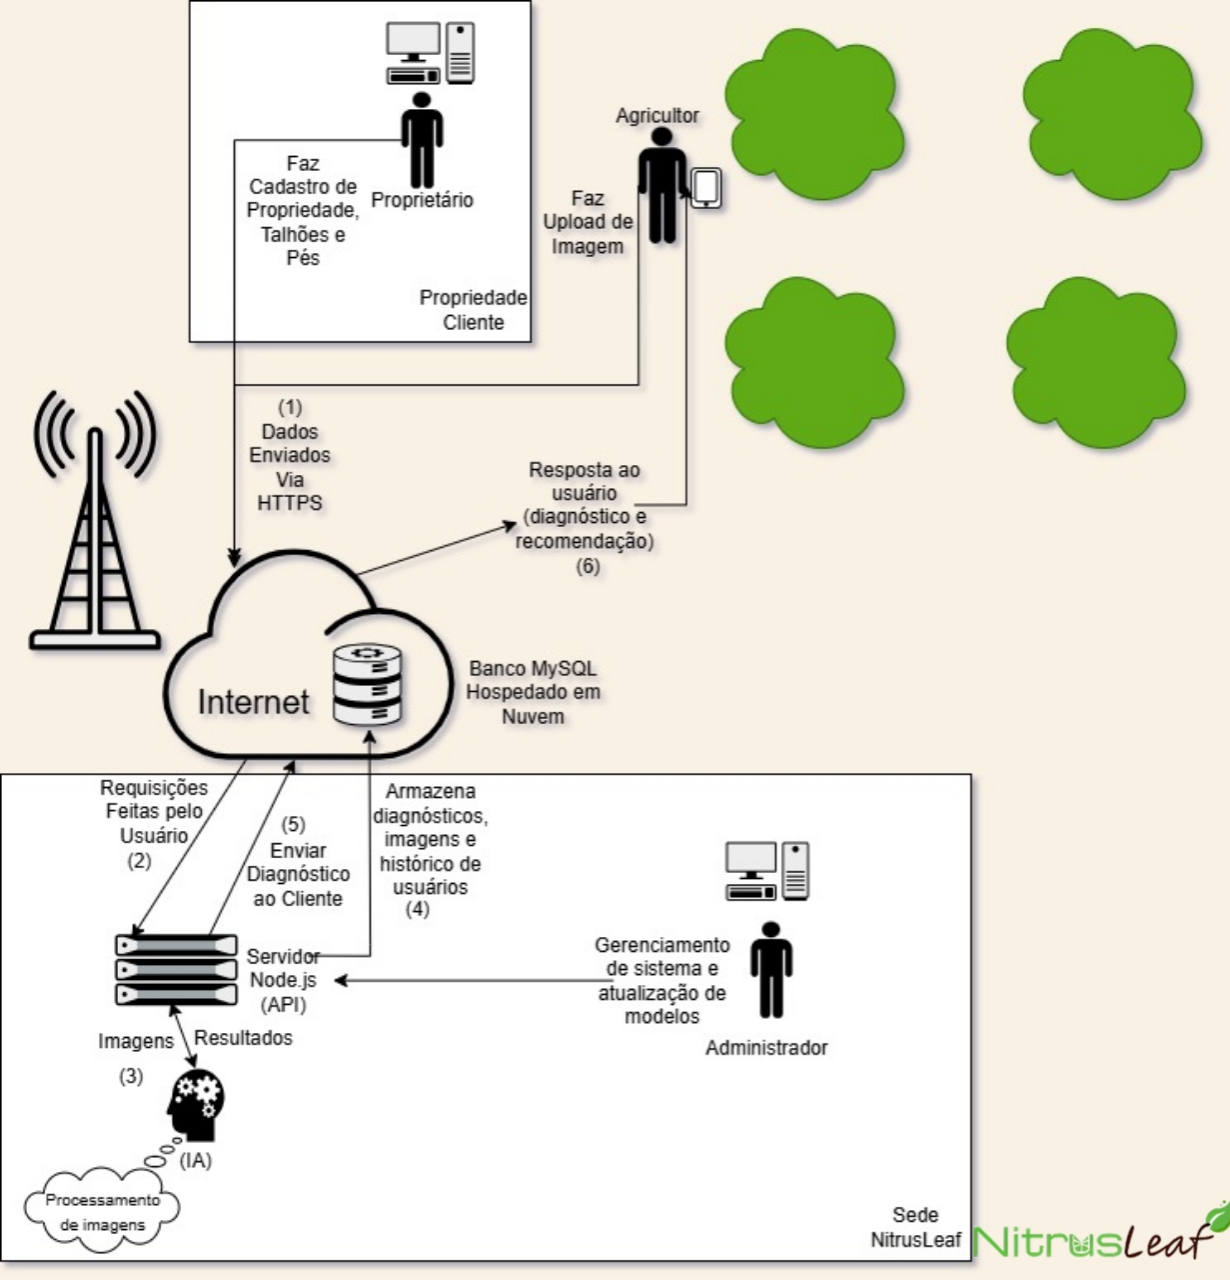
\includegraphics[width=0.8\textwidth]{Images/DiagramaInfraestruturaDeRedes.jpg}
\SourceOrNote{Equipe 21 - Vitalliz (2025)}
\end{figure}
\medskip

A infraestrutura de rede integra clientes à Nuvem via HTTPS para processamento por 
IA e persistência de dados no MySQL, sendo orquestrada por uma API Node.js, o que garante segurança, 
escalabilidade e gestão centralizada.
\medskip

% --- UI de Alta Fidelidade (Figma) ---
\section{Interface de Usuário de Alta Fidelidade (Figma)}
Esta seção apresenta as principais telas do sistema para Web e Mobile, desenvolvidas para os usuários
finais. O sistema foi projetado no Figma com foco na usabilidade, acessibilidade e 
praticidade no monitoramento e análise de deficiências nutricionais nas folhas de mexerica.
\medskip    

% ------------------------------------------------------------------
    \subsection{\textbf{Interface do Usuário - Web}}
    \label{sect:Interface-Web}
    
\begin{figure}[H]
\centering
\caption{Protótipo Interface Web - Tela de Login}
\label{fig:interface-web-tela-login}
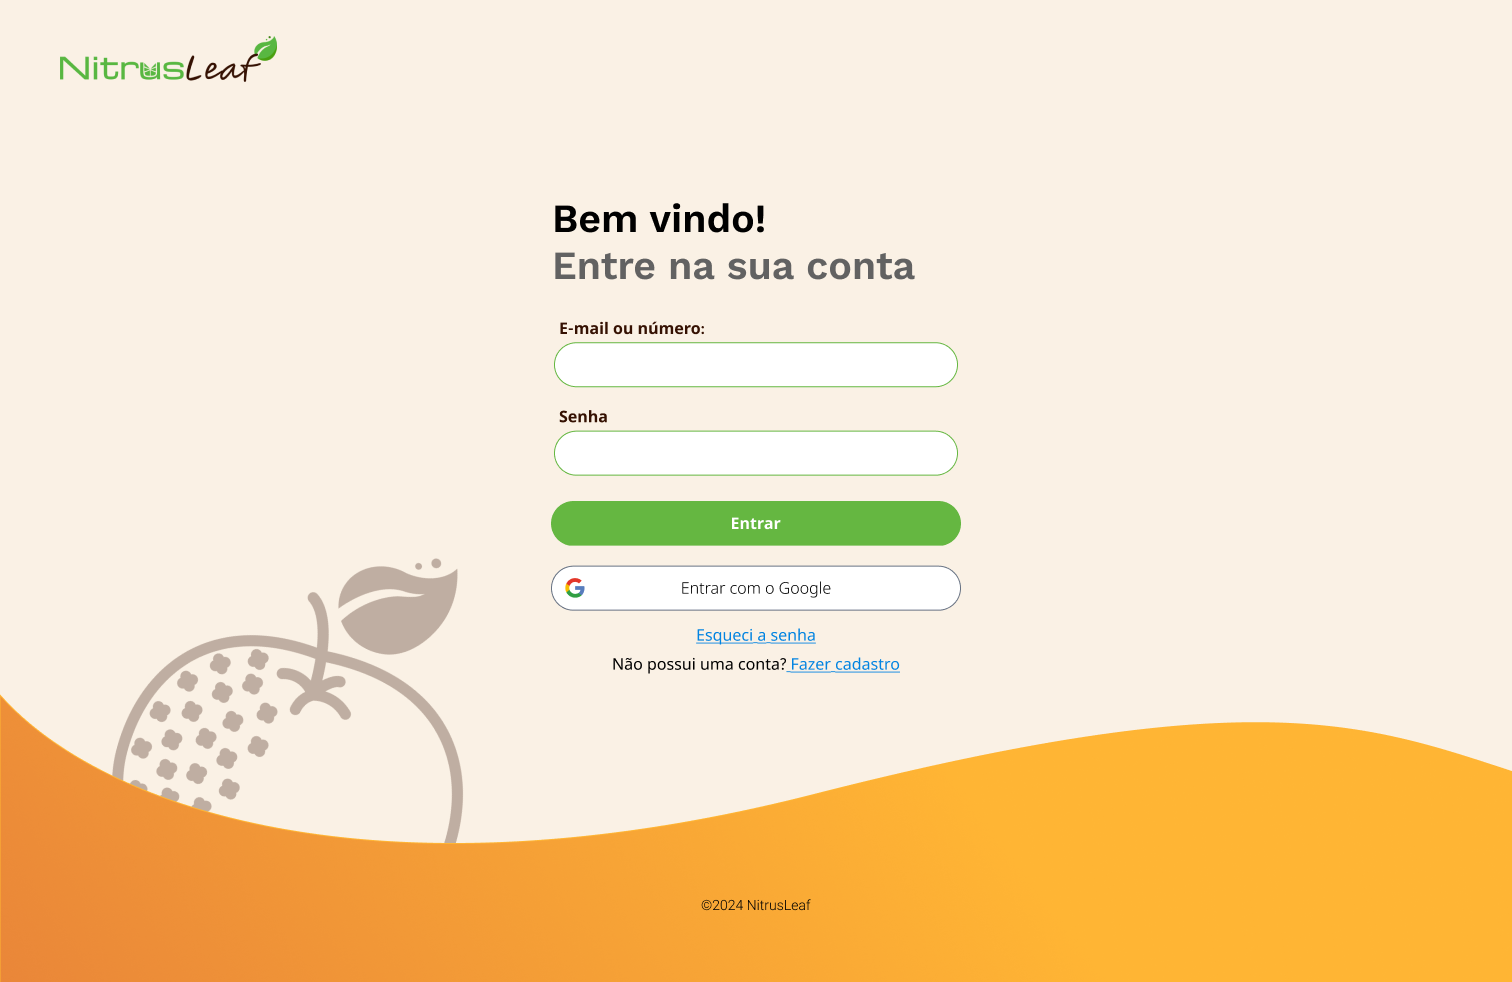
\includegraphics[width=0.8\textwidth]{Images/TelaLogin.png}
\SourceOrNote{Equipe 21 - Vitalliz (2025)}
\end{figure}

A tela de login é o ponto de entrada do sistema. Ela permite o acesso de usuários
previamente cadastrados, garantindo segurança e controle de acesso às
funcionalidades do sistema.
\medskip


\begin{figure}[H]
\centering
\caption{Protótipo Interface Web - Tela de Histórico}
\label{fig:interface-web-telahistorico-1}
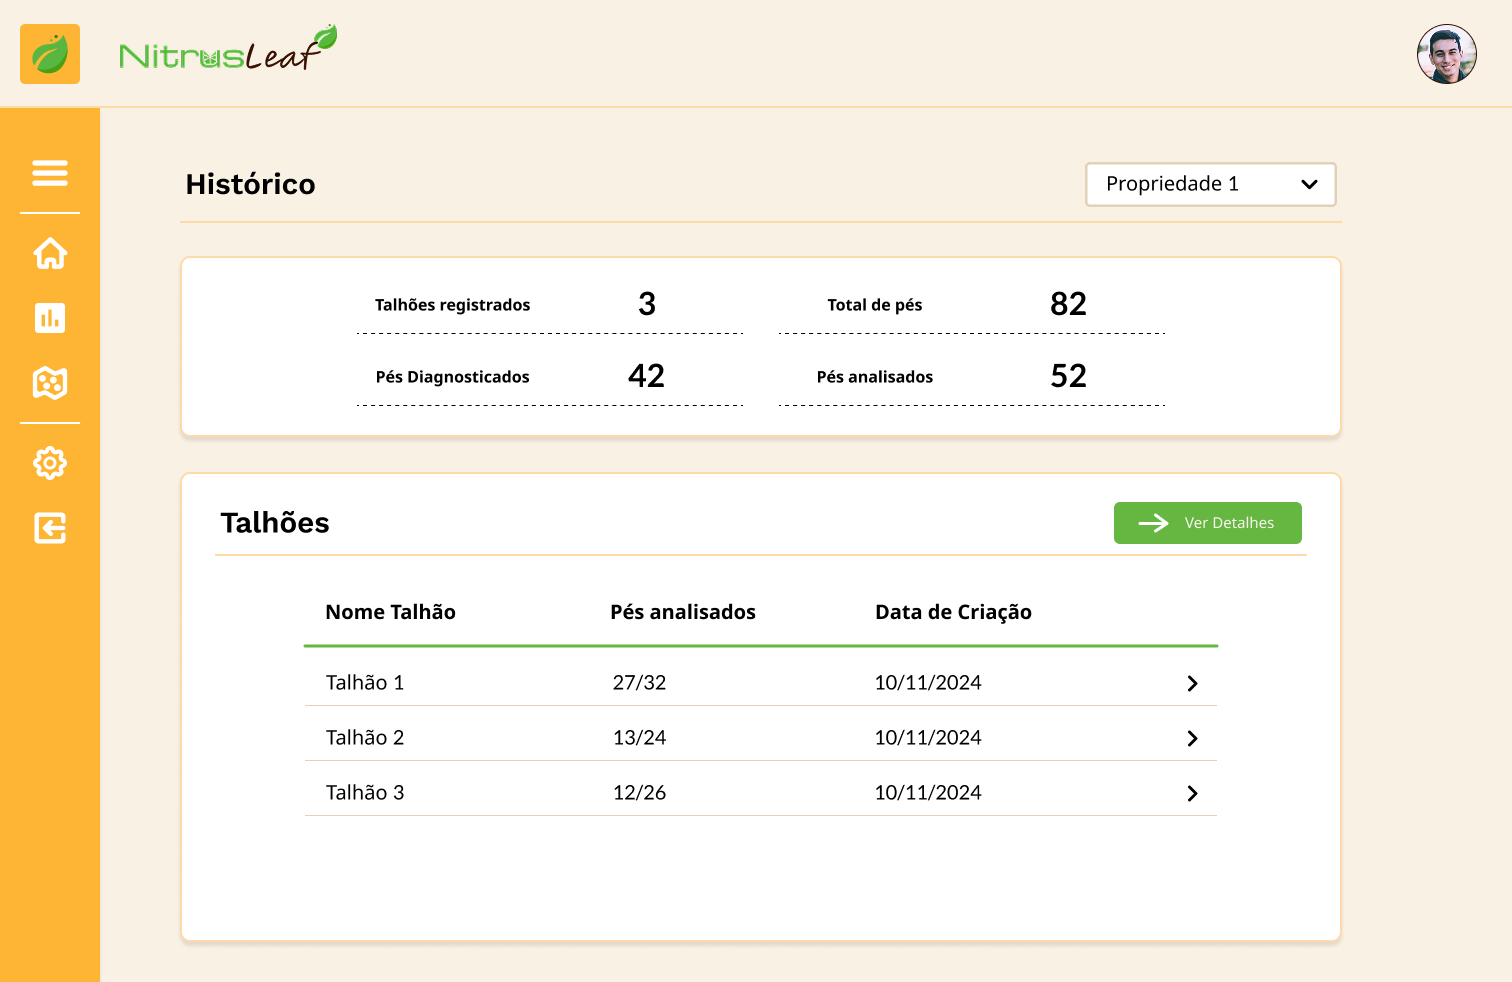
\includegraphics[width=0.8\textwidth]{Images/TelaHistorico-1.png}
\SourceOrNote{Equipe 21 - Vitalliz (2025)}
\end{figure}

A tela de histórico apresenta registros anteriores de análises feitas em cada
talhão, permitindo o acompanhamento da evolução das deficiências identificadas,
datas de envio das imagens e resultados processados.
\medskip


\begin{figure}[H]
\centering
\caption{Protótipo nterface Web - Tela de Resultados}
\label{fig:interface-web-tela-resultados}
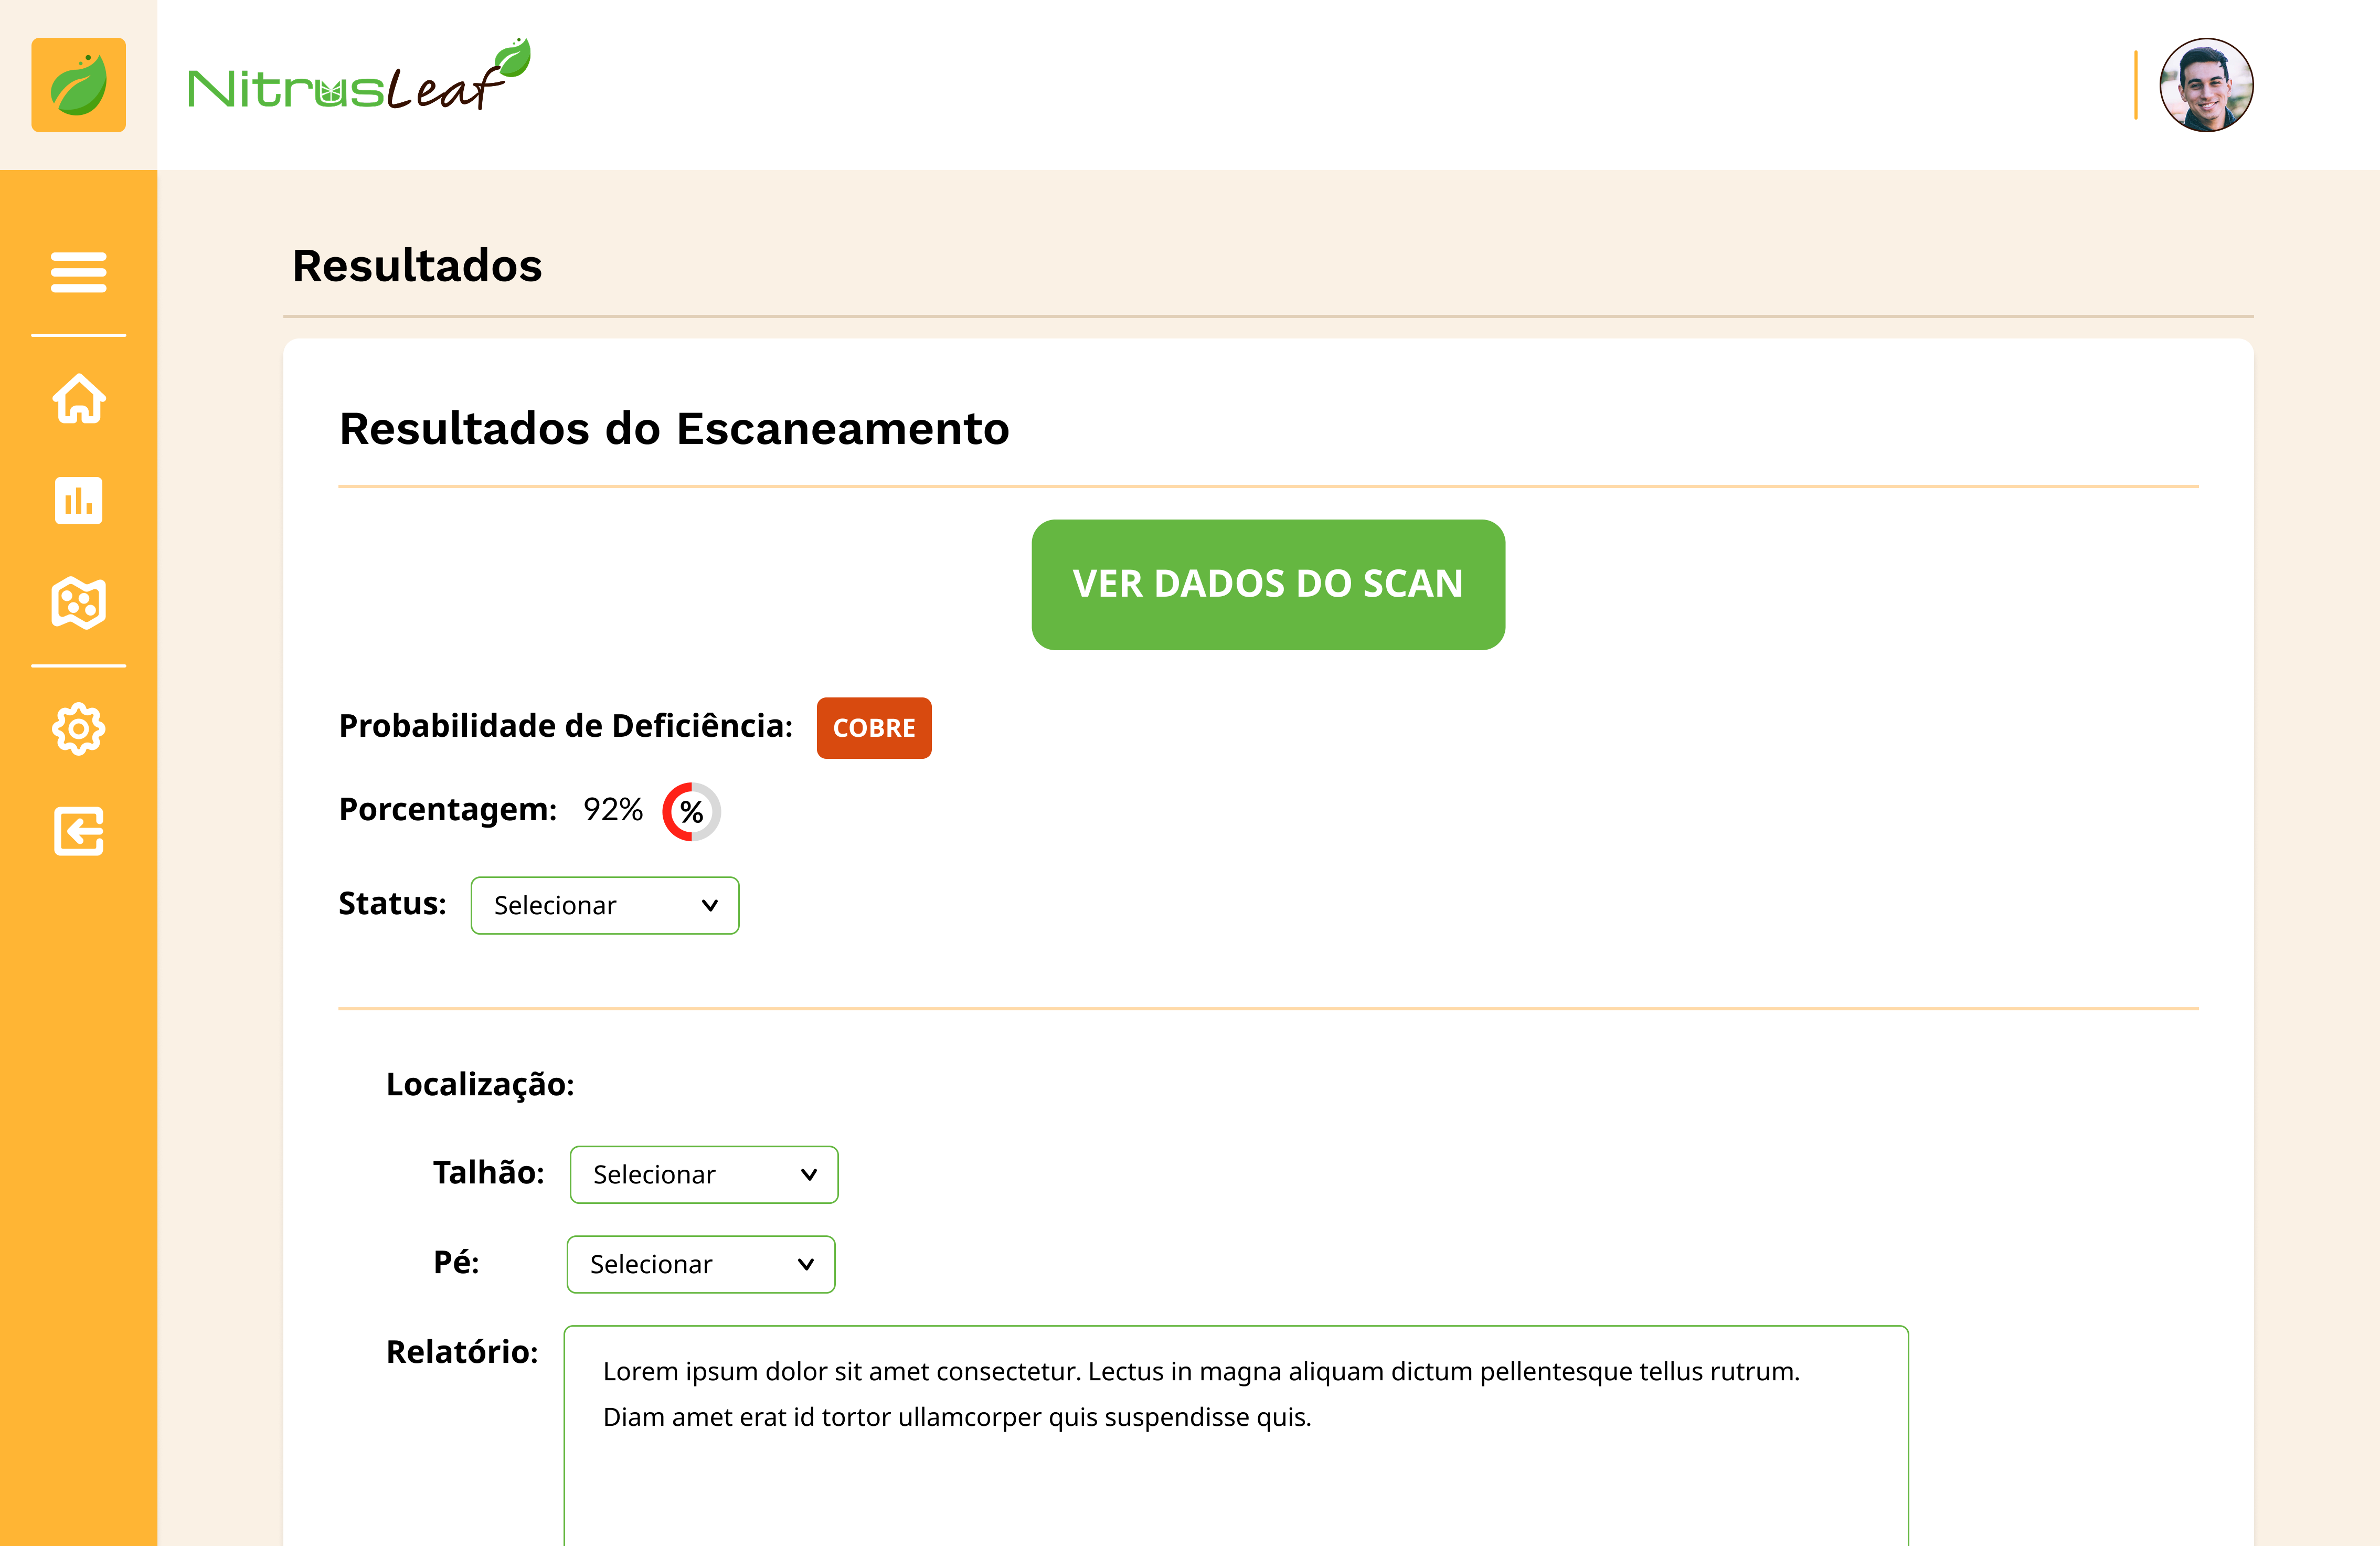
\includegraphics[width=0.8\textwidth]{Images/TelaResultado.png}
\SourceOrNote{Equipe 21 - Vitalliz (2025)}
\end{figure}

A tela de Resultados exibe os resultados detalhados das análises realizadas nas
imagens enviadas, incluindo definição de status e criação de relatórios.
\medskip


\begin{figure}[H]
\centering
\caption{Protótipo Interface Web - Tela de Mapa}
\label{fig:interface-web-tela-mapa}
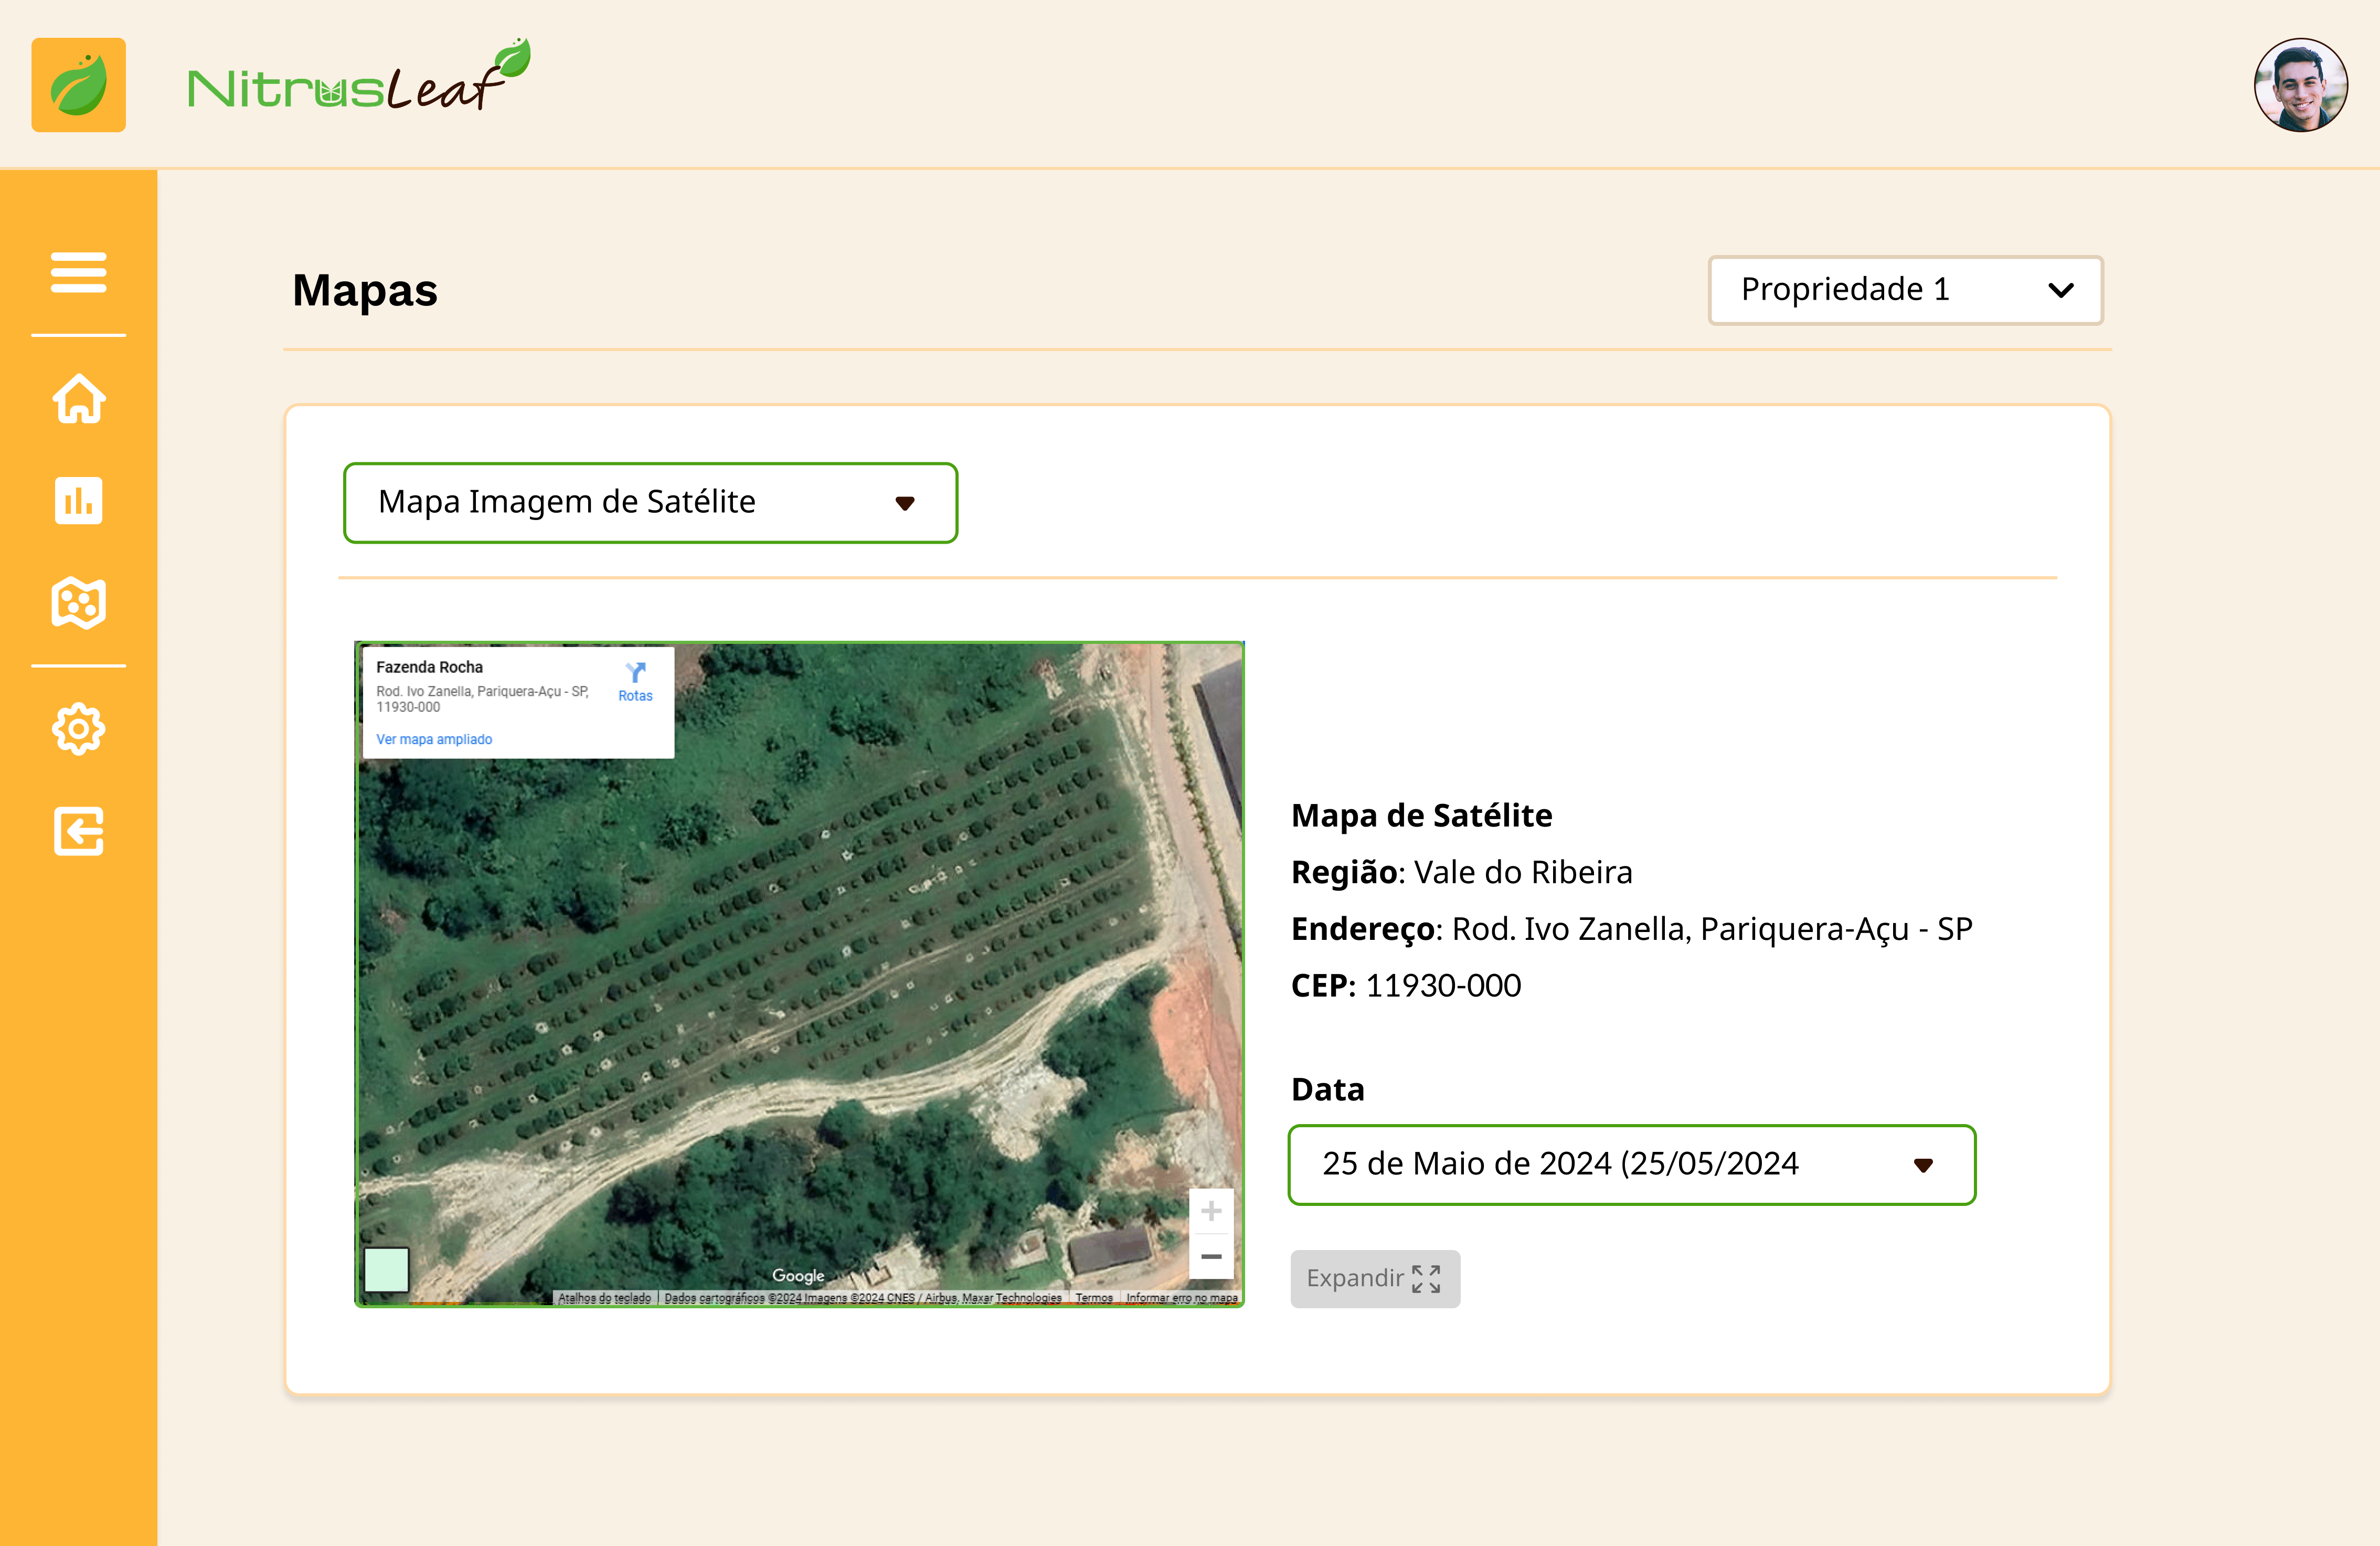
\includegraphics[width=0.8\textwidth]{Images/TelaMapa.png}
\SourceOrNote{Equipe 21 - Vitalliz (2025)}
\end{figure}

Nesta tela, o usuário pode visualizar os talhões de sua propriedade em um
mapa interativo.
\medskip

% ------------------------------------------------------------------
    \subsection{\textbf{Interface do Usuário - Mobile}}
    \label{sect:Interface-Mobile}
    
\begin{figure}[H]
\centering
\caption{Protótipo Interface Mobile - Tela de Login}
\label{fig:interface-mobile-tela-login}
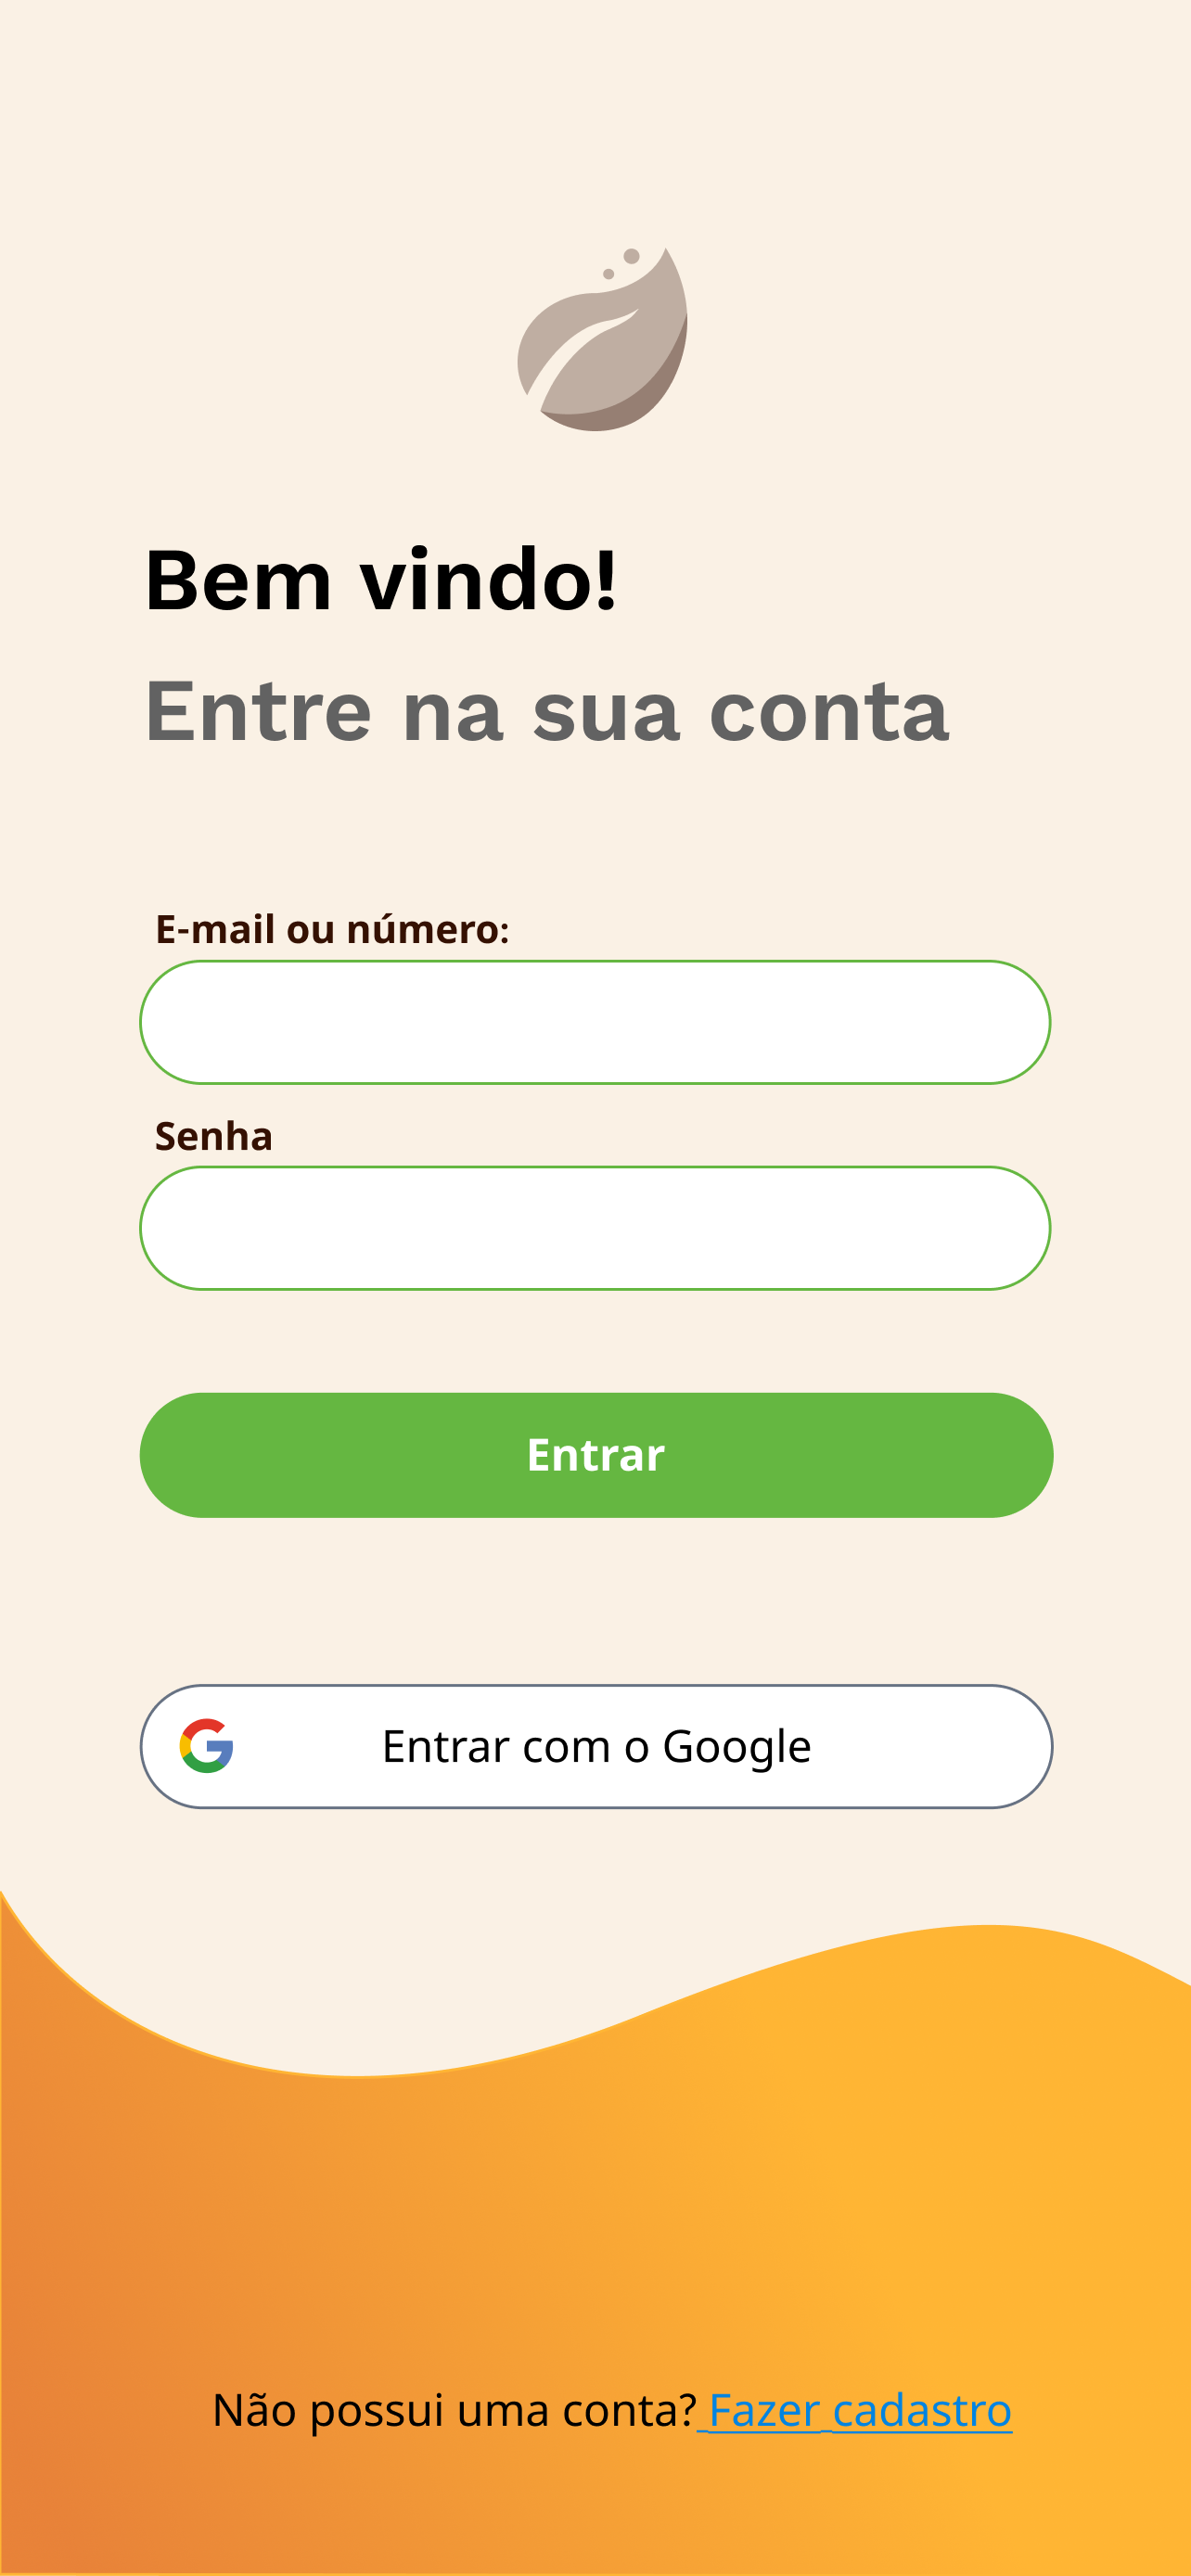
\includegraphics[width=0.2\textwidth]{Images/MobileLogin.png}
\SourceOrNote{Equipe 21 - Vitalliz (2025)}
\end{figure}

A tela de login é o ponto de entrada do sistema. A versão mobile mantem a
funcionalidade e visual da versão web, adaptada para ficar mais agradavel no uso 
de dispositivos móveis.
\medskip


\begin{figure}[H]
\centering
\caption{Protótipo Interface Web - Tela de Início}
\label{fig:interface-web-tela-inicio}
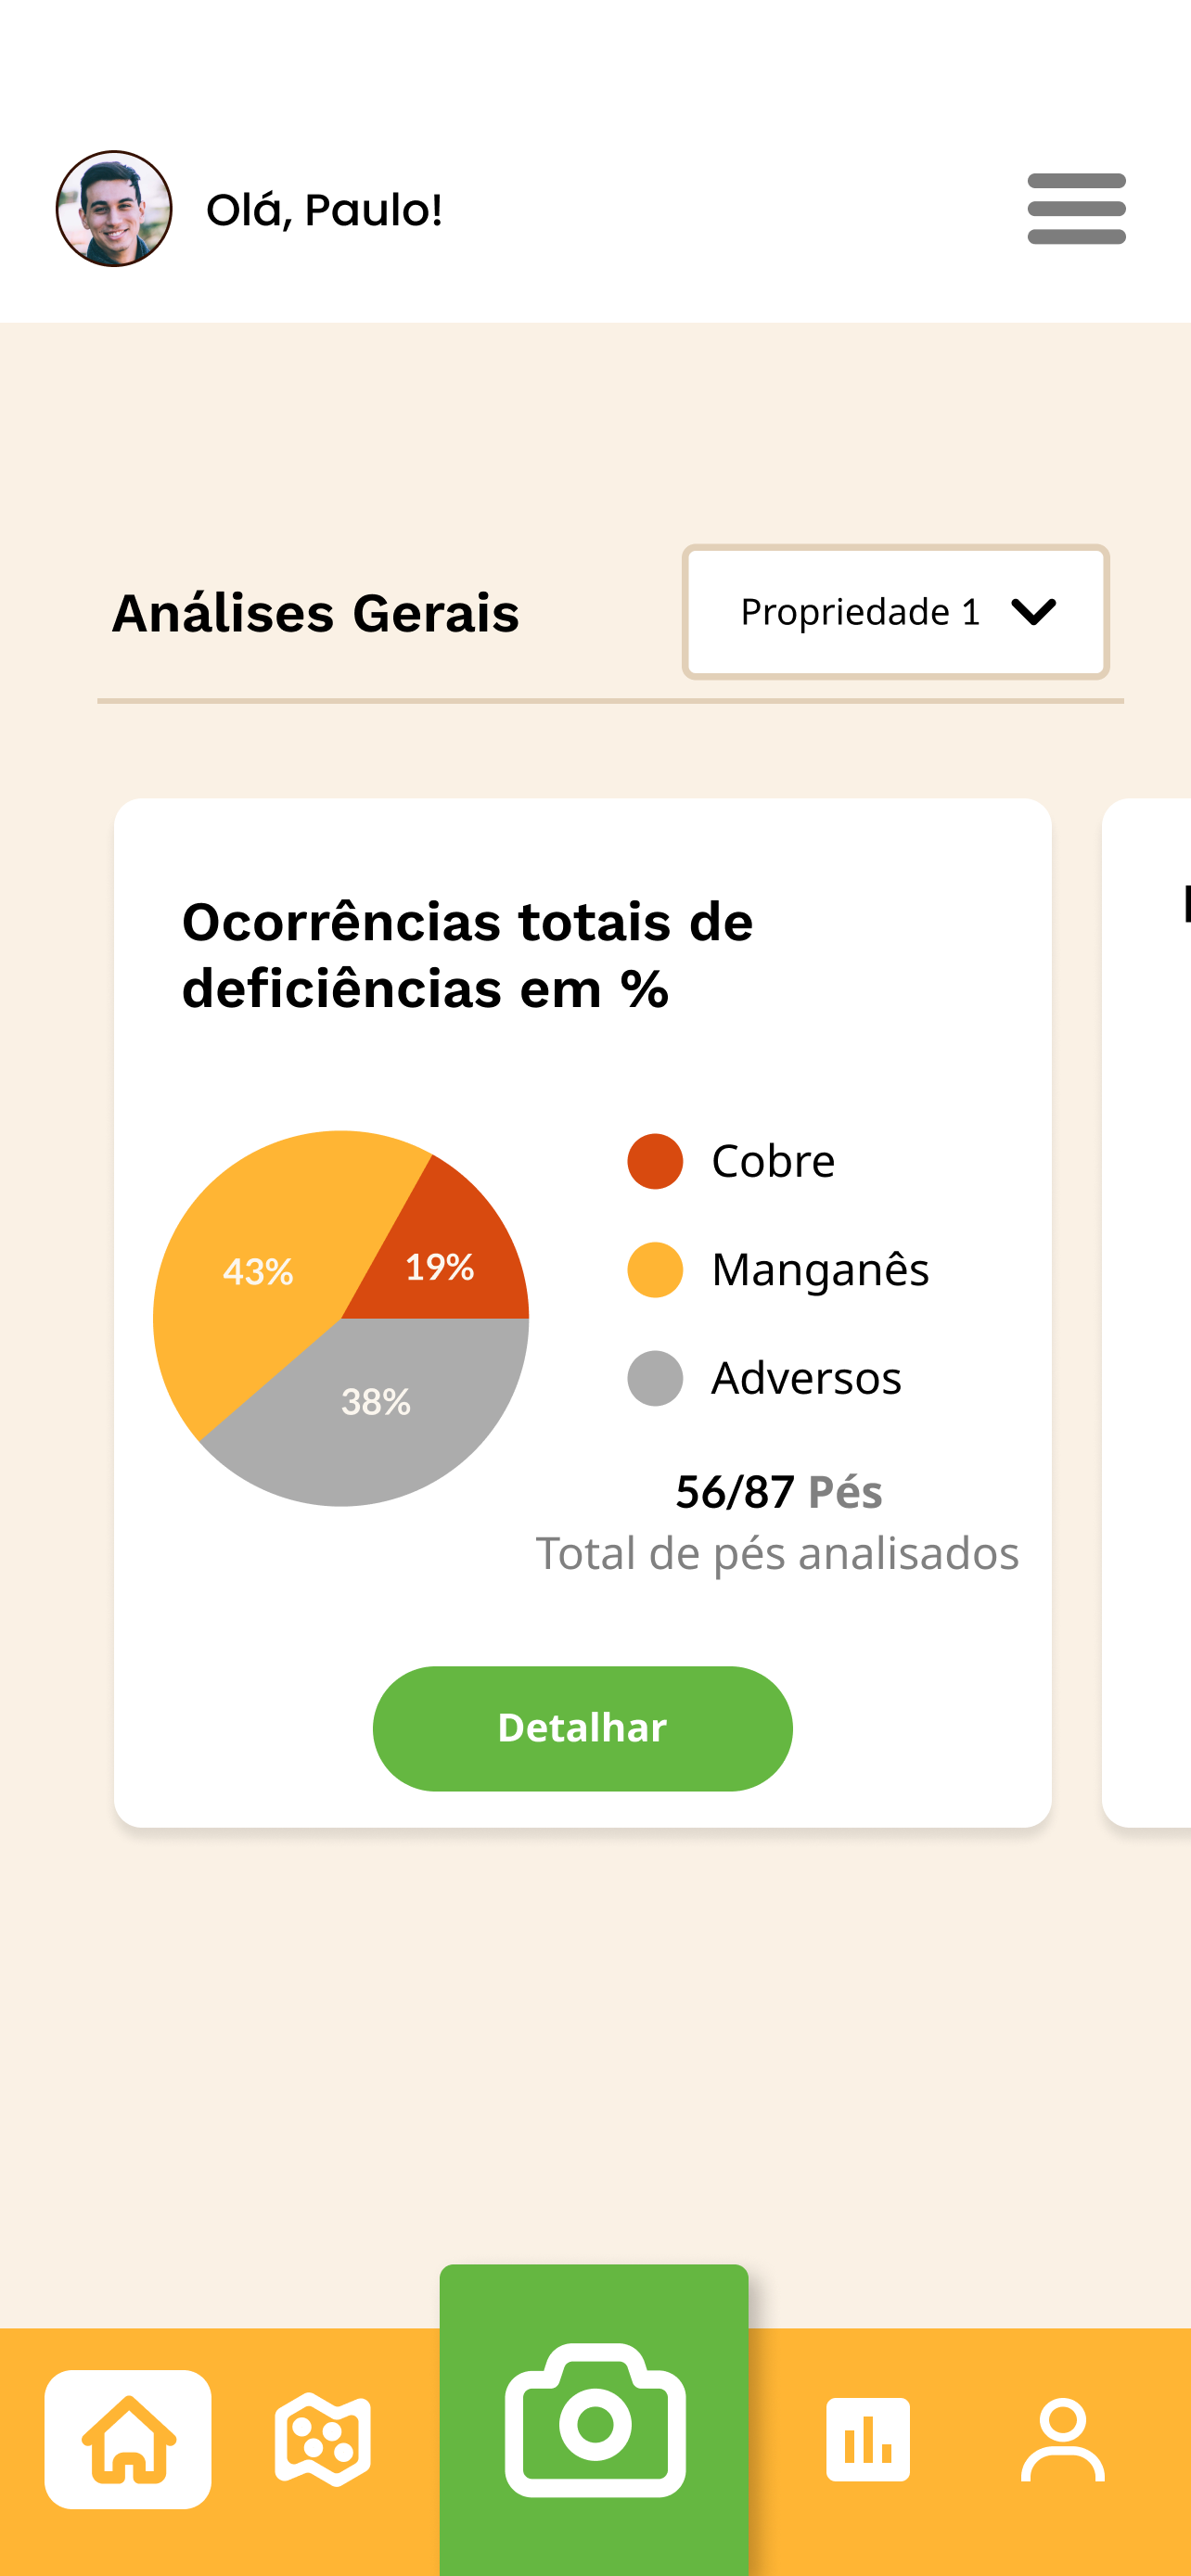
\includegraphics[width=0.2\textwidth]{Images/MobileInicio.png}
\SourceOrNote{Equipe 21 - Vitalliz (2025)}
\end{figure}

O menu inicial mobile apresenta as principais funcionalidades do sistema de forma
otimizada para dispositivos móveis, garantindo fácil acesso e navegação.
\medskip



\begin{figure}[H]
\centering
\caption{Protótipo Interface Web - Tela de Histórico}
\label{fig:interface-web-telahistorico-1}
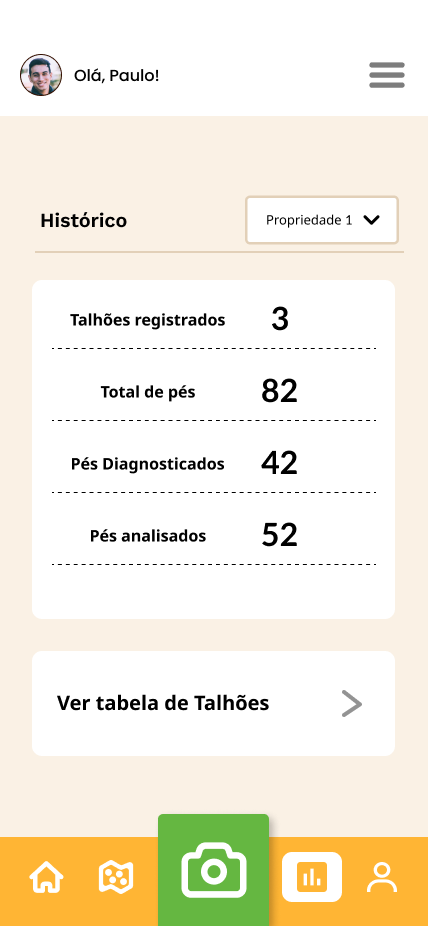
\includegraphics[width=0.2\textwidth]{Images/MobileHistorico.png}
\SourceOrNote{Equipe 21 - Vitalliz (2025)}
\end{figure}

A tela de histórico mobile também apresenta a visão geral das análises e cadastros da 
propriedade, com layout otimizado para telas menores.
\medskip



\begin{figure}[H]
\centering
\caption{Protótipo Interface Mobile - Tela de Resultados}
\label{fig:interface-mobile-tela-resultados}
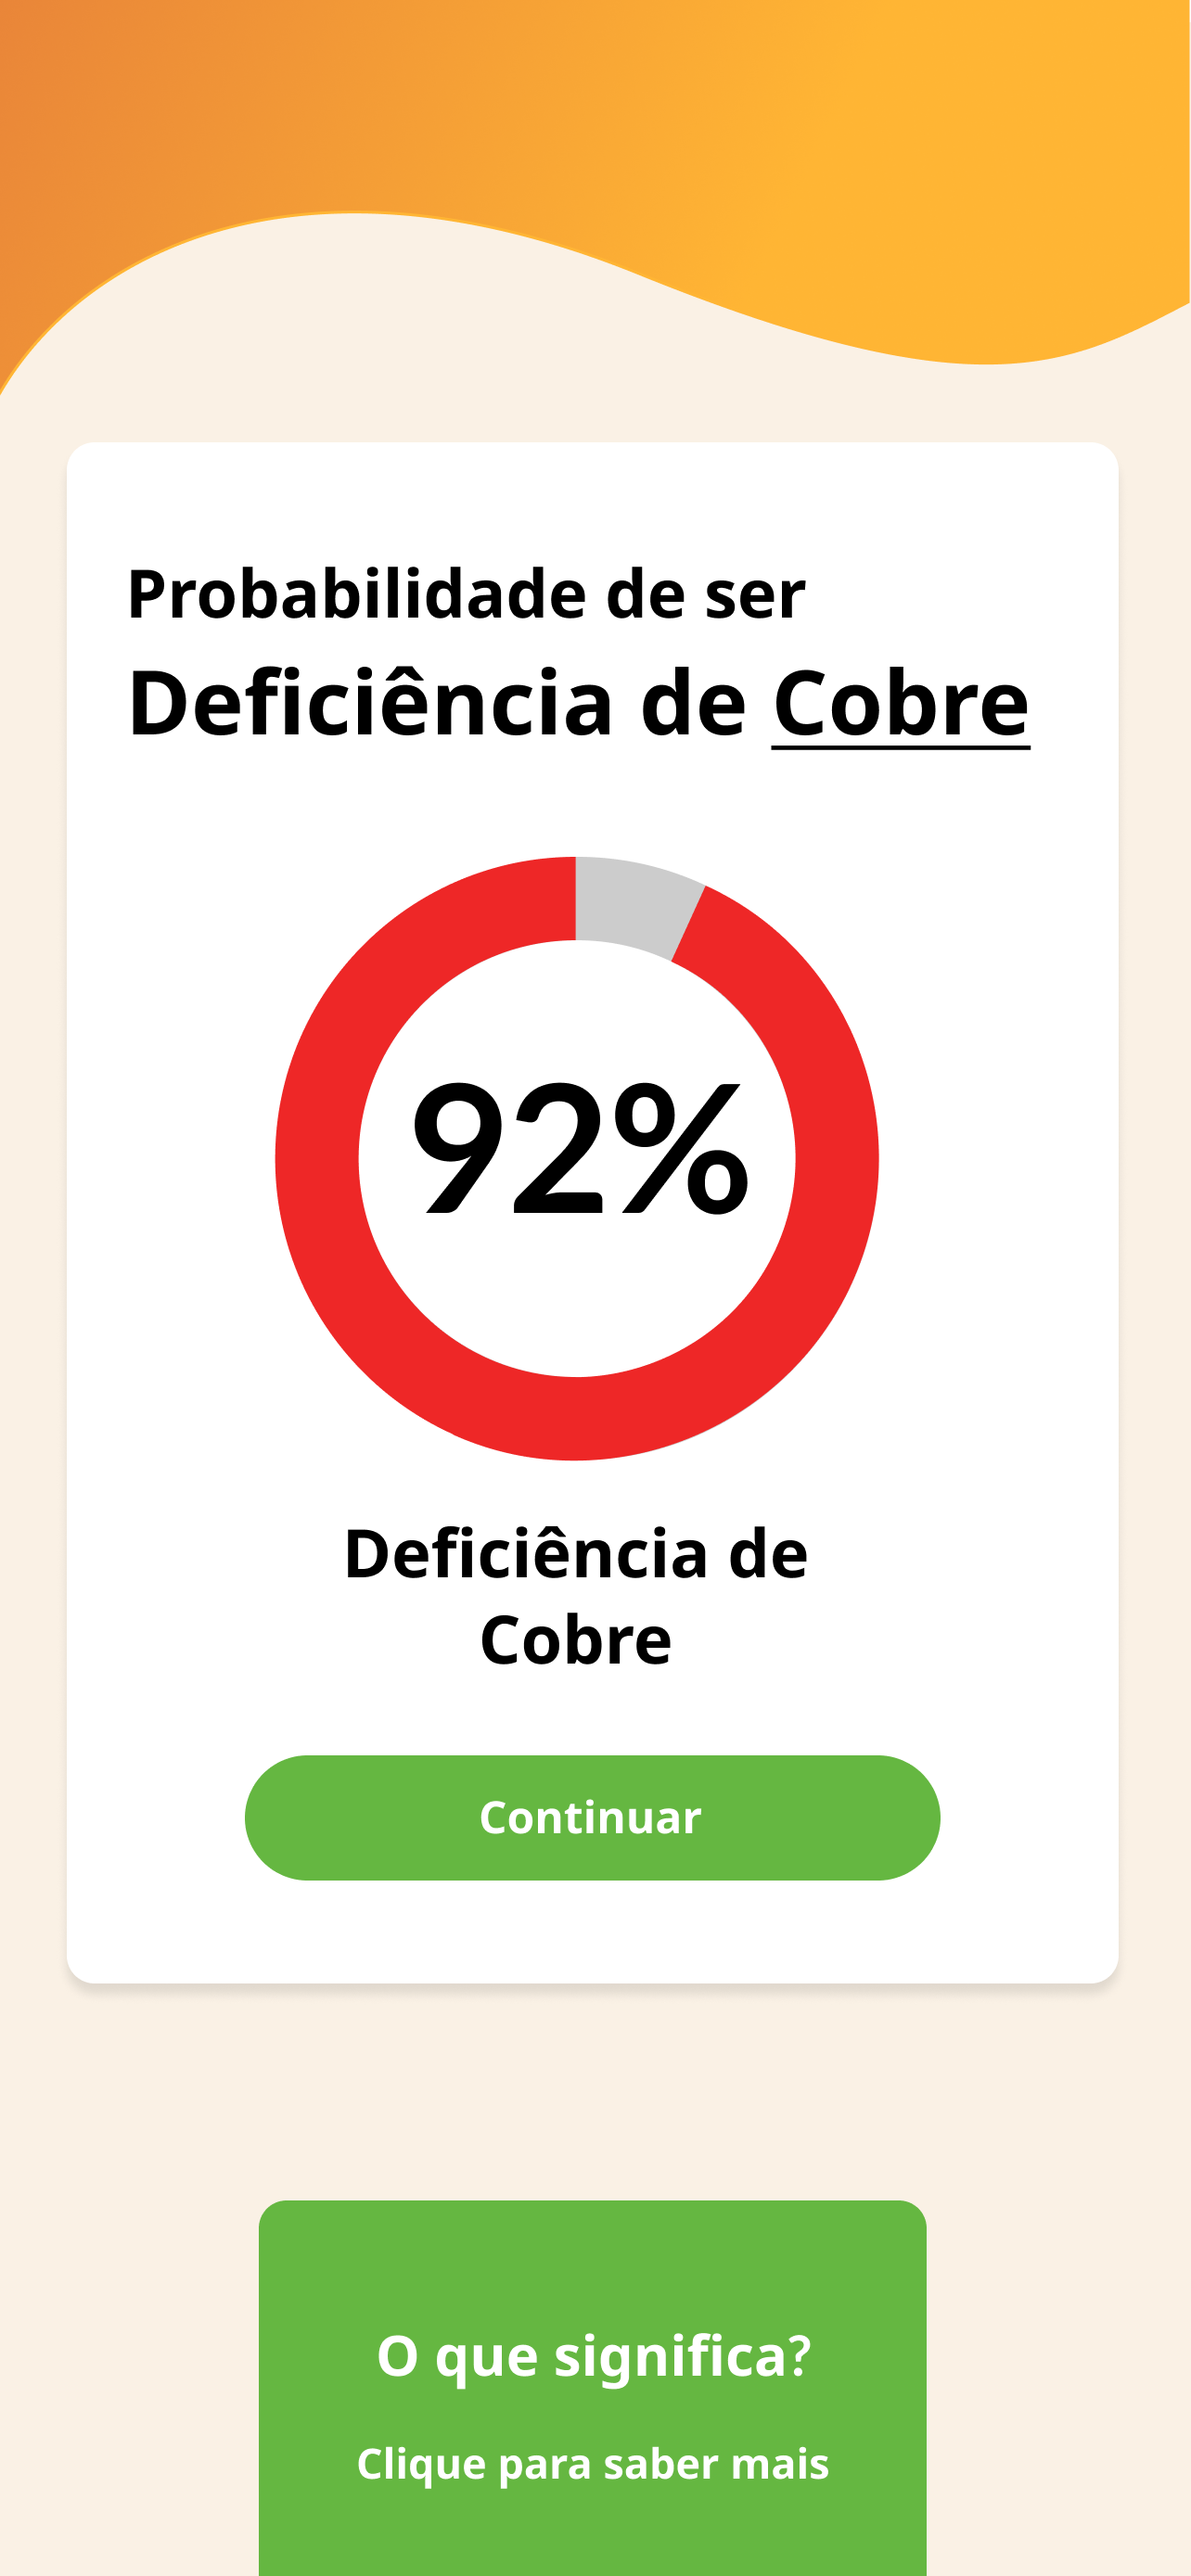
\includegraphics[width=0.2\textwidth]{Images/MobileResultado.png}
\SourceOrNote{Equipe 21 - Vitalliz (2025)}
\end{figure}

A tela de Resultados exibe os resultados detalhados das análises realizadas na
imagem enviada, permitindo melhor visualização do diagnóstico.
\medskip


\begin{figure}[H]
\centering
\caption{Protótipo Interface Mobile - Tela de Mapa}
\label{fig:interface-mobile-tela-mapa}
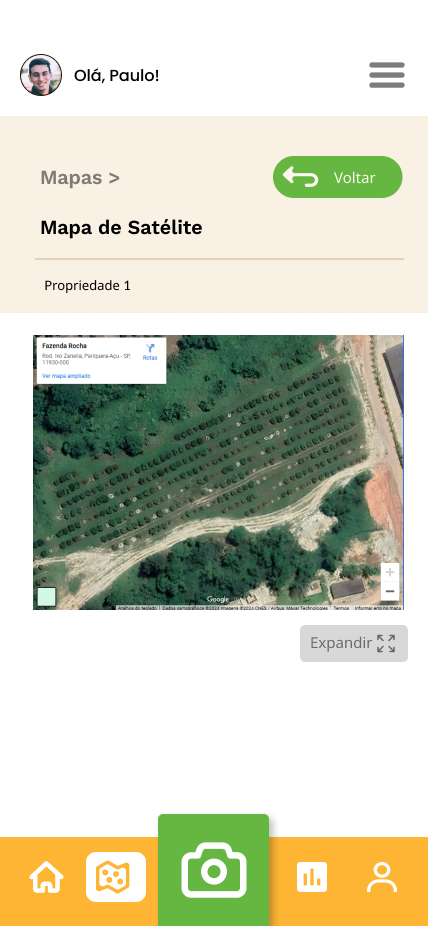
\includegraphics[width=0.2\textwidth]{Images/MobileMapa.png}
\SourceOrNote{Equipe 21 - Vitalliz (2025)}
\end{figure}

Nesta tela, o usuário pode visualizar os talhões de sua propriedade em um
mapa interativo.
\medskip

% --- Interface da Aplicação ---
\section{Interface da Aplicação}
\medskip
    \label{sect:Interface-Aplicacao}
    Esta seção apresenta as principais telas do sistema Web desenvolvidas em Node.js
(Express + Sequelize) com MySQL e EJS. Esta versão não possui todas as funcionalidades
finais, mas demonstra a estrutura básica e a navegação entre as páginas, além do funcionamento
do banco de dados.
\medskip

\begin{figure}[H]
\centering
\caption{Interface Web - Tela de Login}
\label{fig:interface-web-tela-login}
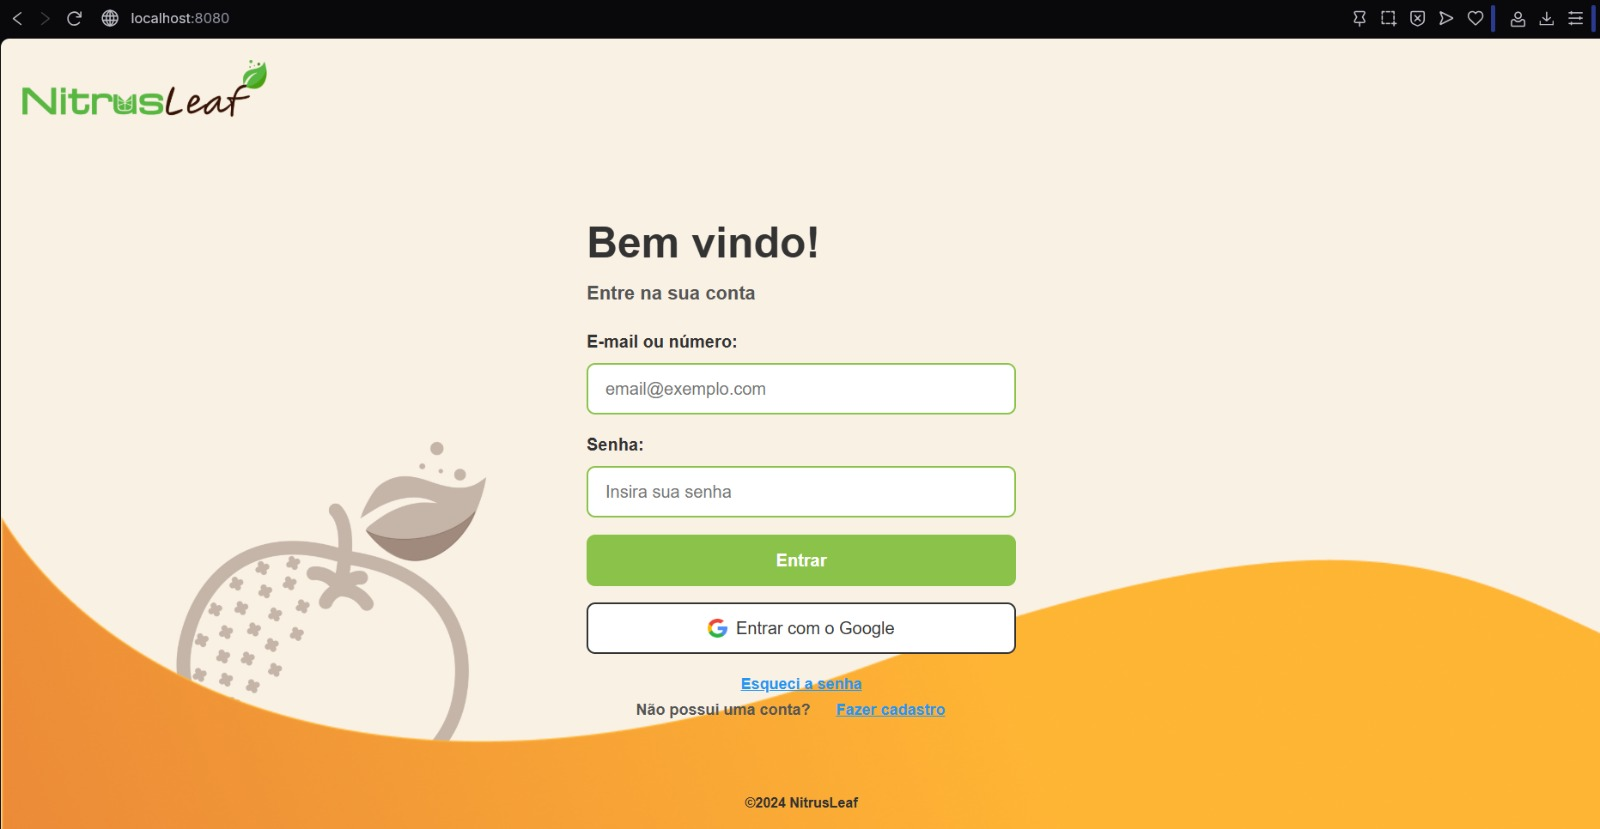
\includegraphics[width=0.8\textwidth]{Images/AppLogin.png}
\SourceOrNote{Equipe 21 - Vitalliz (2025)}
\end{figure}

A tela de login está fiel ao protótipo, com margem para 
ajustes futuros de UX/UI. A autenticação foi implementada via middleware, 
reforçando a segurança.

\begin{figure}[H]
\centering
\caption{Interface Web - Tela de Início}
\label{fig:interface-web-tela-inicio}
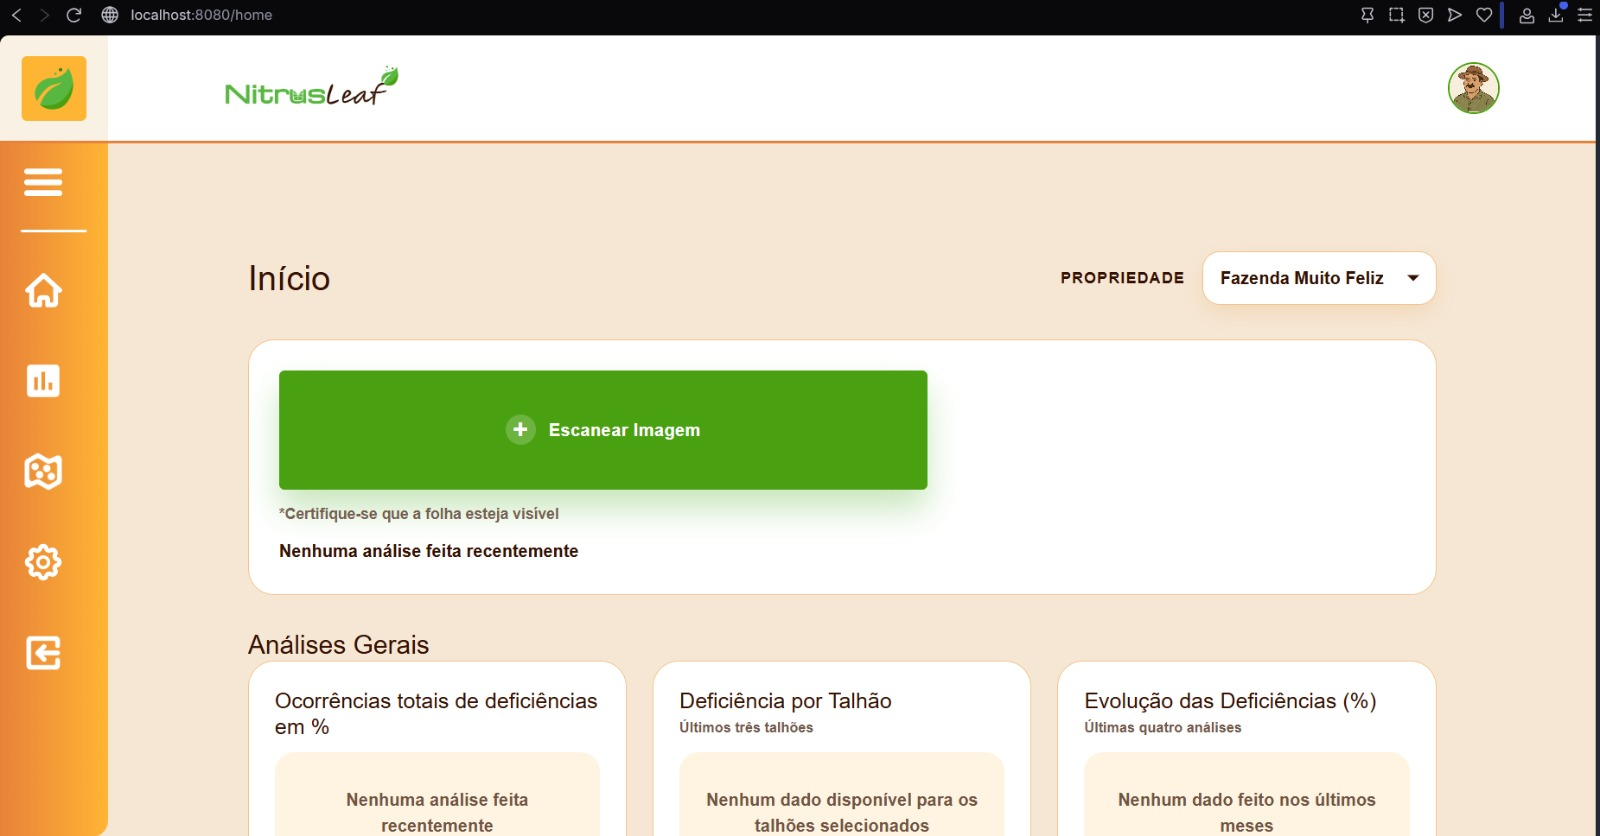
\includegraphics[width=0.8\textwidth]{Images/AppInicio.jpeg}
\SourceOrNote{Equipe 21 - Vitalliz (2025)}
\end{figure}

A tela de início é a primeira tela que o usuário vê após fazer login no sistema. 

\medskip

\begin{figure}[H]
\centering
\caption{Interface Web - Tela de Resultados}
\label{fig:interface-web-tela-resultados}
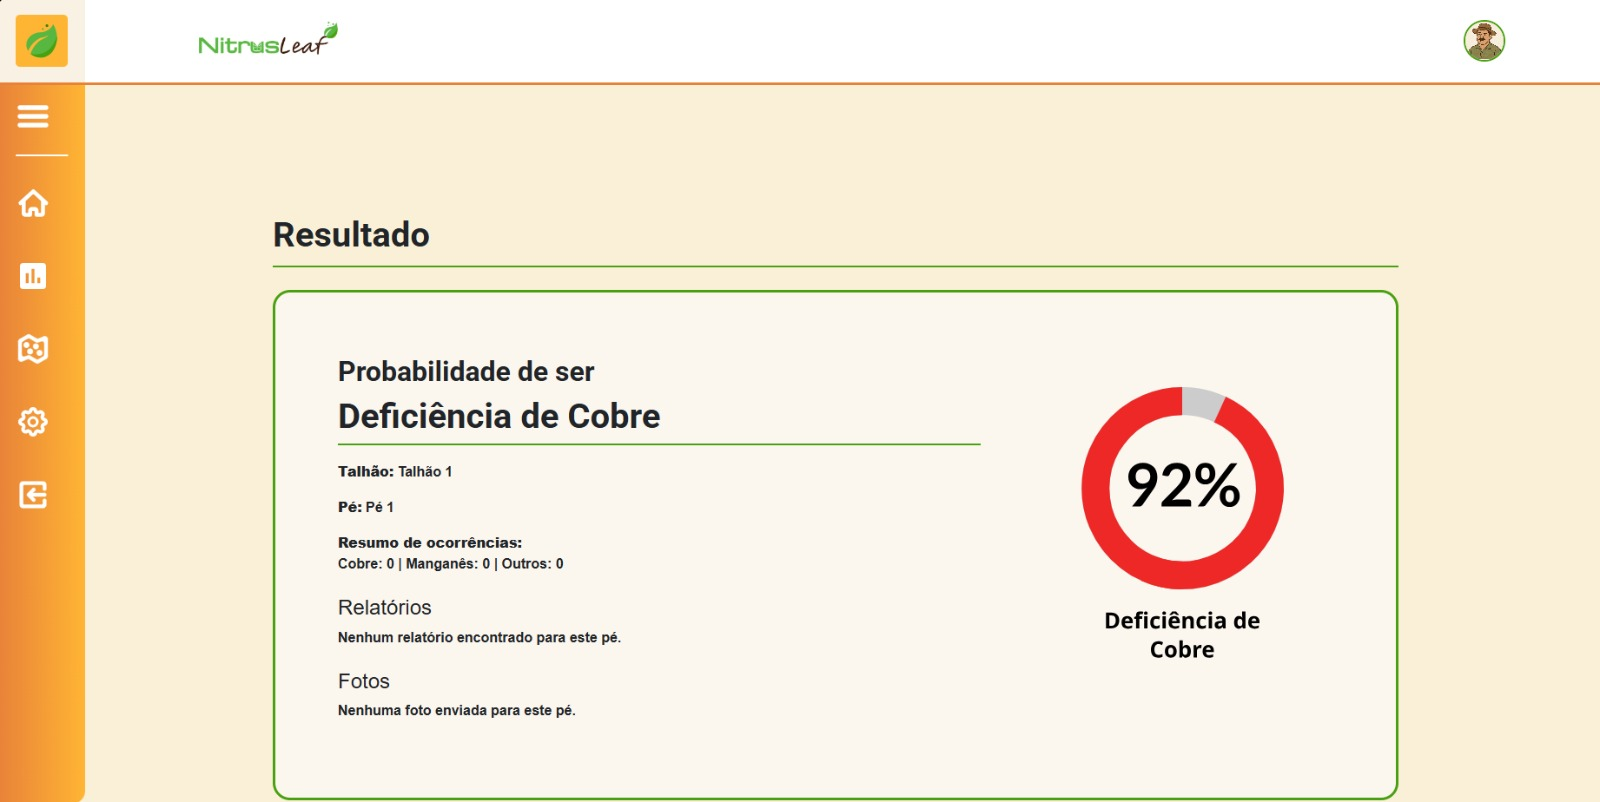
\includegraphics[width=0.8\textwidth]{Images/AppResultado.jpeg}
\SourceOrNote{Equipe 21 - Vitalliz (2025)}
\end{figure}

A tela de Resultados exibe os resultados detalhados das análises realizadas na
imagem enviada, permitindo melhor visualização do diagnóstico.
\medskip

\begin{figure}[H]
\centering
\caption{Interface Web - Tela de Histórico}
\label{fig:interface-web-tela-historico}
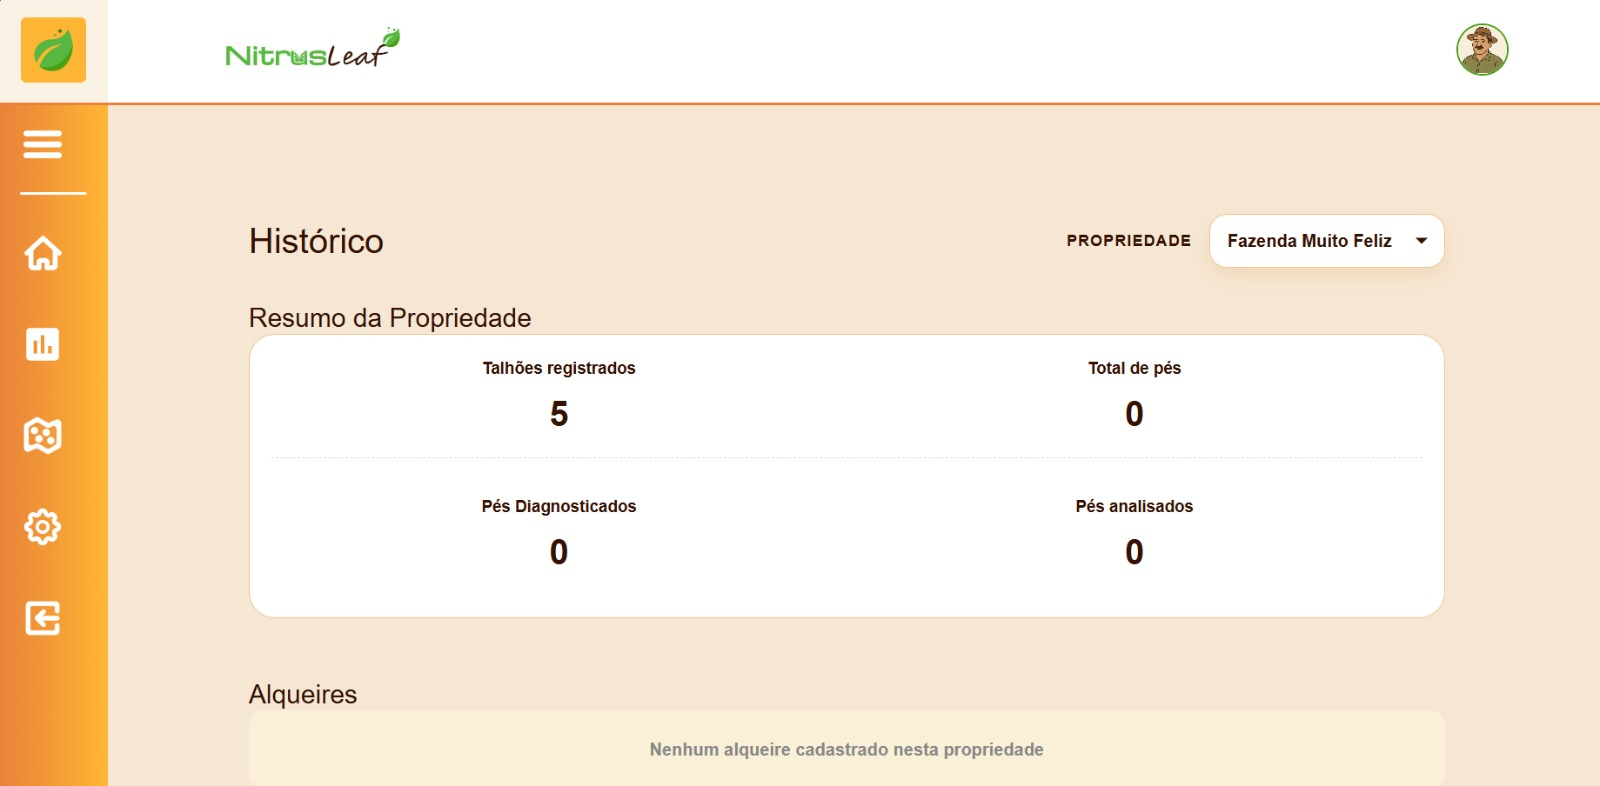
\includegraphics[width=0.8\textwidth]{Images/AppHistorico.jpeg}
\SourceOrNote{Equipe 21 - Vitalliz (2025)}
\end{figure}

A tela de histórico permite que o usuário visualize suas interações anteriores com o sistema, 
facilitando o acompanhamento de suas atividades e resultados ao longo do tempo.
\medskip


\begin{figure}[H]
\centering
\caption{Interface Web - Tela de Mapa}
\label{fig:interface-web-tela-mapa}
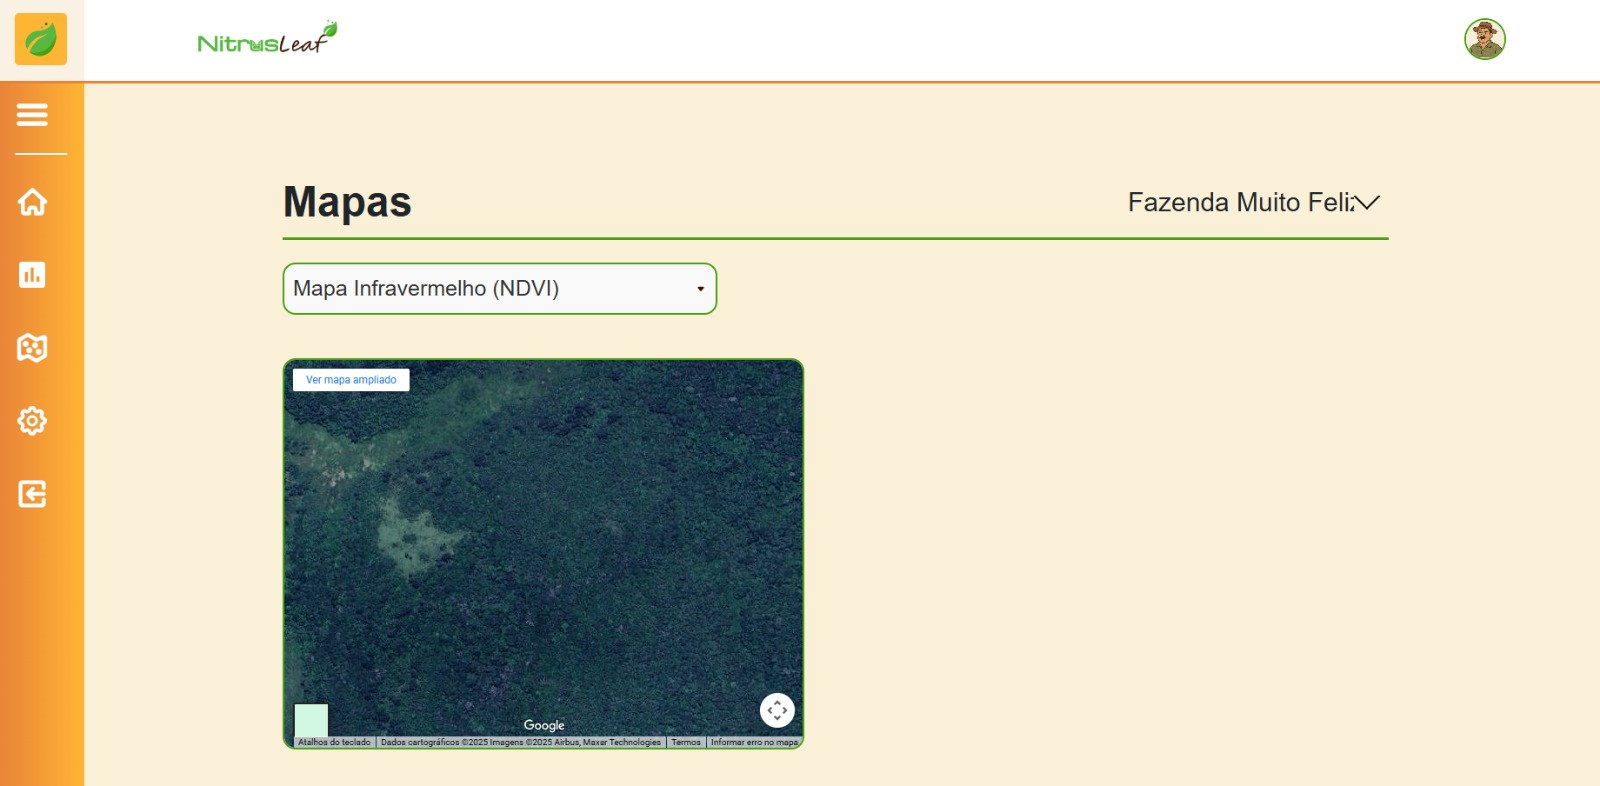
\includegraphics[width=0.8\textwidth]{Images/AppMapa.jpeg}
\SourceOrNote{Equipe 21 - Vitalliz (2025)}
\end{figure}

A tela de mapa permite que o usuário visualize a localização geográfica da propriedade.
\medskip

    

% --- ORGANIZAÇÃO DO PROJETO COM SCRUM ---
\section{Organização do Projeto com Scrum}
\medskip
    \label{sect:Scrum}
    Para organizar as atividades de desenvolvimento deste projeto, optamos por utilizar
a metodologia ágil \textbf{Scrum}. Com ela, foi possível dividir as entregas em tarefas
específicas, acompanhar o progresso do time e garantir o cumprimento dos prazos
definidos.
\medskip


\noindent{As tarefas foram organizadas em três colunas principais:}
\begin{itemize}[itemsep=0.6em, topsep=0.3em, parsep=0pt]
    \item \textbf{Pendente}:  Tarefas ainda não iniciadas;
    \item \textbf{Em Progresso}: Tarefas que estão sendo desenvolvidas no momento;
    \item \textbf{Concluído}: Tarefas já finalizadas pela equipe.
\end{itemize}
\medskip

\begin{figure}[H]
\centering
\caption{Quadro Scrum com tarefas do projeto}%
\label{fig:quadro-scrum}
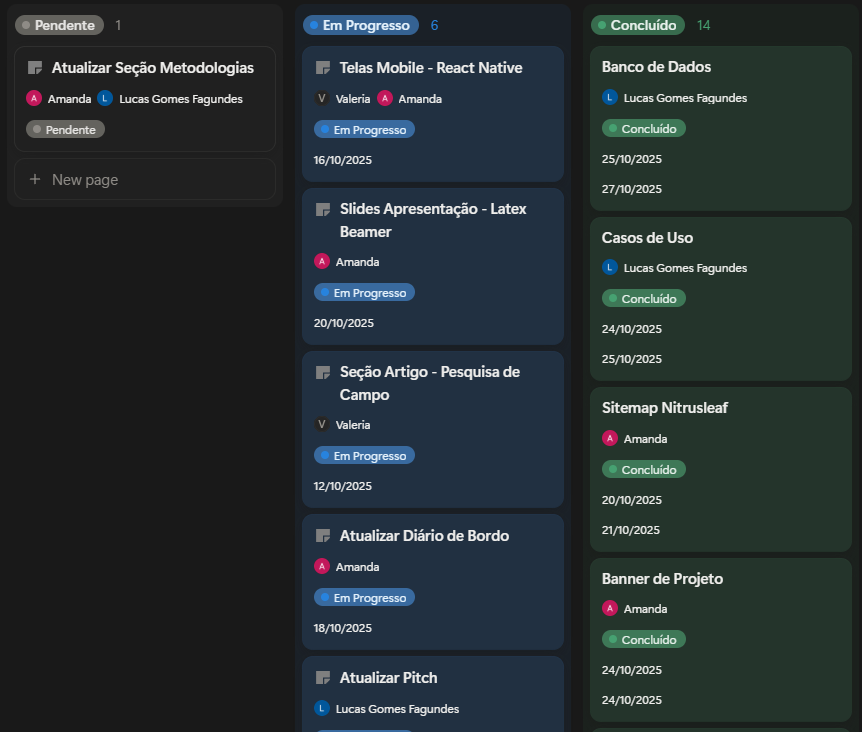
\includegraphics[width=0.8\textwidth]{Images/Scrum.png}
\SourceOrNote{Equipe 21 - Vitalliz (2025)}
\end{figure}
\medskip

Cada atividade foi priorizada conforme sua urgência e atribuída aos membros
responsáveis. Essa abordagem nos permitiu manter o foco, colaborar de forma
eficiente e adaptar o projeto conforme as necessidades surgiam ao longo do tempo.


% --- DIÁRIO DE BORDO ---
\section{Diário de Bordo}
\medskip
    \label{sect:Diario-de-Bordo}
    Durante os três semestres de desenvolvimento anteriores, realizamos diversas
atividades que contribuíram para a construção e evolução do projeto. Abaixo,
apresentamos imagens detalhadas sobre cada etapa durante os semestres:

% -- 1° Semestre --
\begin{center}
\captionof{table}{Diário de Bordo – 2º Semestre}
\begin{adjustbox}{max width=\textwidth}
\begin{tabular}{|m{4cm}|m{2.5cm}|m{2.5cm}|m{3cm}|m{8cm}|}
\hline
\textbf{Nome da Atividade} &
\textbf{Data de Início} &
\textbf{Data de Término} &
\textbf{Responsável pela Atividade} &
\textbf{Descrição da Atividade Realizada} \\ \hline

Pesquisa temas para o Projeto & 27/02/2024 & 09/03/2024 & Atividade realizada em grupo &
Realizamos pesquisas para possíveis temas, resultando como escolhido o tema Identificação de deficiência de manganês e cobre na folha da mexerica. \\ \hline

Pesquisas de artigos científicos & 10/03/2024 & 16/03/2024 & Atividade realizada em grupo &
Realizamos pesquisas de artigos científicos para fortalecer o desenvolvimento do tema. \\ \hline

Elaboração do artigo & 17/03/2024 & 19/03/2024 & Atividade realizada em grupo &
Cada um ficou responsável por desenvolver um tópico do artigo se baseando nas pesquisas e reuniões em grupo. \\ \hline

Introdução & 20/03/2024 & 18/04/2024 & Luiz &
Realização da introdução do artigo científico. \\ \hline

Objetivo & 20/03/2024 & 18/04/2024 & Amanda Vithória &
Realização do tópico objetivo do artigo científico. \\ \hline

Estado da Arte & 20/03/2024 & 18/04/2024 & Lucas &
Realização do Estado da Arte do artigo científico. \\ \hline

Metodologia & 20/03/2024 & 18/04/2024 & Valéria &
Realização da metodologia do artigo científico. \\ \hline

Criação do manual de identidade visual & 31/03/2024 & 21/04/2024 & Atividade realizada em grupo &
Como proposto na aula de design, deveríamos elaborar um manual para representar a identidade visual do nosso projeto e da nossa equipe. \\ \hline

Criação das logos & 31/03/2024 & 05/04/2024 & Lucas e Amanda Vithória &
Elaborar as logos da equipe e do projeto. \\ \hline

Escolha das paletas de cores & 06/04/2024 & 08/04/2024 & Decisão tomada em grupo &
Escolher as cores que estarão no projeto. \\ \hline

Escolha da tipografia & 08/04/2024 & 10/04/2024 & Decisão tomada em grupo &
Escolher as tipografias que estarão no projeto. \\ \hline

Apresentação do manual de identidade visual & 22/04/2024 & 22/04/2024 & -- &
Apresentação do manual de identidade visual. \\ \hline

Modelo de baixa fidelidade do Figma & 23/04/2024 & 26/04/2024 & Valéria &
Estruturamos o modelo da aplicação que mostra quais telas são necessárias e quais elementos são importantes para seu funcionamento, norteando o design e auxiliando no banco de dados do projeto. \\ \hline

Modelo conceitual de banco de dados & 25/04/2024 & 30/04/2024 & Valéria &
O modelo conceitual é responsável por definir entidades e o relacionamento entre elas, norteando como o sistema deve funcionar. \\ \hline

Modelo de Alta Fidelidade & 28/04/2024 & 01/06/2024 & Amanda Vithória &
Estruturar o modelo da aplicação que mostra com detalhes como cada tela vai funcionar. Nesse processo, as telas irão servir como uma prévia final de aplicação, demonstrando a interação do usuário com o sistema. \\ \hline

Oracle APEX do projeto & 06/05/2024 & 01/06/2024 & Luiz &
Responsável por mostrar um site que exibe as telas previstas no projeto mais desenvolvido, incluindo mapa, mapa de calor e gráficos com quantidade de incidências e não incidências. \\ \hline

Diagrama de Redes & 13/05/2024 & 20/05/2024 & Lucas e Luiz &
O diagrama de redes mostra como a infraestrutura do projeto irá funcionar. \\ \hline

Diagrama de Caso de Uso & 13/05/2024 & 20/05/2024 & Amanda e Luiz &
O diagrama de caso de uso mostra os processos que ocorrem durante a utilização do software. \\ \hline

Site da Equipe & 13/05/2024 & 27/05/2024 & Lucas &
O site descreve um pouco da equipe, mostrando o nicho de atuação dos integrantes e uma breve descrição do projeto. \\ \hline

Banner & 20/05/2024 & 03/06/2024 & Amanda Vithória &
O banner demonstra de forma resumida todo o projeto para apresentações ao público. \\ \hline

\end{tabular}
\end{adjustbox}

\vspace{0.3em}
\small{\textbf{Fonte:} Equipe 21 – Vitalliz (2024)}

\end{center}

% -- 2° Semestre --
\begin{center}
\captionof{table}{Diário de Bordo – 2º Semestre}
\begin{adjustbox}{max width=\textwidth}
\begin{tabular}{|m{4cm}|m{2.2cm}|m{2.2cm}|m{3cm}|m{8cm}|}
\hline
\textbf{Nome da Atividade} &
\textbf{Data de Início} &
\textbf{Data de Término} &
\textbf{Responsável pela Atividade} &
\textbf{Descrição da Atividade Realizada} \\ 
\hline

Revisão do Artigo & 08/10/2024 & 17/11/2024 & Luiz &
Foram corrigidos erros de português, revisados os objetivos e reformulada a seção de estado da arte. Além disso, incluíram-se os resultados preliminares com as telas do site, o modelo físico do banco de dados e explicações sobre o diagrama de classes e objetos na seção de resultados. Por fim, algoritmos de recursividade foram implementados na tela de busca do site. \\ \hline

Prototipação das Telas do Site no Figma & 05/10/2024 & 17/11/2024 & Amanda &
Desenvolvimento das telas iniciais com base na prototipação do semestre anterior, incluindo as telas da versão mobile, com adição de landing page e reformulação do design anterior para a versão desktop web. Foram criados componentes para reduzir o número de telas e tornar o desenvolvimento mais eficiente, além de aprimorar o design para facilitar a visualização da simulação. \\ \hline

Desenvolvimento da Parte Front-End do Site & 15/10/2024 & 17/11/2024 & Amanda e Valéria &
Criação das telas web seguindo fielmente as telas prototipadas no Figma. O desenvolvimento do design foi feito utilizando CSS e Bootstrap, mantendo o layout responsivo e visualmente coerente com o projeto. \\ \hline

Desenvolvimento da Parte Back-End do Site & 15/10/2024 & 17/11/2024 & Todos os integrantes do grupo &
Foram implementadas as funcionalidades do protótipo criado no Figma, incluindo sistemas internos de rota e integração com o banco de dados. Foram utilizadas bibliotecas e funcionalidades do Node.js, como Express, Nodemon, Middleware, View Engine EJS e Sequelize (para integração com MySQL2). A arquitetura MVC foi adotada para estruturar melhor as pastas e organizar o código. \\ \hline

Banco de Dados Físico & 25/10/2024 & 10/11/2024 & Lucas &
Criação do banco de dados utilizado no site, estruturado conforme todas as funcionalidades previstas no projeto, garantindo coerência entre o modelo físico e os requisitos do sistema. \\ \hline

Diagrama de Entidade-Relacionamento (DER) & 23/10/2024 & 25/10/2024 & Lucas &
O DER do banco de dados foi refeito, incluindo todos os dados corretos e alinhados com a versão atual do projeto, garantindo consistência e completude no modelo conceitual. \\ \hline

Diagrama de Classe & 25/09/2024 & 17/11/2024 & Luiz &
Elaboração do diagrama de classes do projeto, com base nas funções implementadas. O diagrama representa a estrutura de classes e suas relações, definindo atributos e métodos de cada componente do sistema. \\ \hline

Diagrama de Objetos & 25/09/2024 & 17/11/2024 & Luiz &
Criação do diagrama de objetos, representando instâncias concretas das classes principais do projeto e demonstrando as interações entre elas. \\ \hline

Diagrama de Caso de Uso & 11/11/2024 & 17/11/2024 & Valéria &
Refação do diagrama de caso de uso, contemplando todos os atores e suas respectivas ações, alinhadas com as funcionalidades atuais do sistema. \\ \hline

Banner & 13/11/2024 & 18/11/2024 & Amanda &
Desenvolvimento do banner do projeto, que será utilizado na próxima feira tecnológica, com foco na identidade visual e clareza na apresentação das informações. \\ \hline

\end{tabular}
\end{adjustbox}

\vspace{0.3em}
\small{\textbf{Fonte:} Equipe 21 – Vitalliz (2024)}

\end{center}

% -- 3° Semestre --
\begin{center}
\captionof{table}{Diário de Bordo – 3º Semestre}
\begin{adjustbox}{max width=\textwidth}
\begin{tabular}{|m{4cm}|m{2.2cm}|m{2.2cm}|m{3cm}|m{8cm}|}
\hline
\textbf{Nome da Atividade} &
\textbf{Data de Início} &
\textbf{Data de Término} &
\textbf{Responsável pela Atividade} &
\textbf{Descrição da Atividade Realizada} \\ 
\hline

Diagrama de Banco de Dados Conceitual (DER) & 18/02/2025 & 28/02/2025 & Luiz &
Refação completa do banco de dados, iniciando pelo Diagrama Entidade-Relacionamento (DER). O banco foi reestruturado para alinhar com as exigências e requisitos do projeto, otimizando o armazenamento de dados. \\ \hline

Diagrama de Banco de Dados Lógico (MER) & 09/03/2025 & 10/03/2025 & Valéria &
Elaboração do Modelo Entidade-Relacionamento Lógico (MER), baseado no DER. A estrutura foi ajustada para garantir a integridade e eficiência do banco de dados, atendendo aos requisitos do sistema. \\ \hline

Modelo Físico do Banco & 18/02/2025 & 28/02/2025 & Luiz &
Desenvolvimento do Modelo Físico do Banco de Dados, aplicando as definições do DER e MER. A modelagem física define os tipos de dados e as tabelas de armazenamento para otimizar a consulta e performance do sistema. \\ \hline

Revisão do Artigo & 31/03/2025 & 11/05/2025 & Luiz &
Revisão do artigo conforme o feedback recebido na última banca. A introdução foi reescrita para ser mais concisa, evitando redundâncias e abordando de maneira mais objetiva os pontos principais. O objetivo foi aprimorado de acordo com as orientações dos professores, melhorando sua clareza e alinhamento com o escopo do projeto. Pequenos ajustes foram feitos na metodologia e no estado da arte. \\ \hline

Análise SWOT & 20/04/2025 & 11/05/2025 & Valéria &
Realização da análise SWOT para identificar as forças, fraquezas, oportunidades e ameaças do projeto. A análise foi conduzida para melhor compreender os pontos fortes e fracos da solução proposta, além de mapear as oportunidades que podem ser aproveitadas e as ameaças que precisam ser mitigadas. Esse processo ajudou a ajustar o planejamento estratégico, proporcionando uma visão mais clara dos desafios e das vantagens competitivas do projeto. \\ \hline

Scrum & 20/04/2025 & 11/05/2025 & Valéria &
Aplicação do framework Scrum para organizar o projeto em sprints, com reuniões de planejamento, acompanhamento e revisão, garantindo agilidade e melhor controle das entregas. \\ \hline

Revisão do Pitch & 09/04/2025 & 19/04/2025 & Lucas &
Revisão do pitch de apresentação, incluindo a tradução das legendas para o inglês, a fim de ampliar a acessibilidade e alcançar um público internacional. Também foi feita a atualização das telas, substituindo as anteriores pelas versões mais recentes do sistema, refletindo o progresso atual do projeto. \\ \hline

Revisão da Logo da Equipe & 17/04/2025 & 30/04/2025 & Amanda &
A logo da equipe foi revista e reformulada para melhorar sua estética visual. A nova versão busca uma representação mais moderna e atrativa, alinhada com a identidade do projeto e com a proposta de inovação tecnológica. Além de melhorar a aparência, o design foi ajustado para garantir maior clareza e legibilidade, mantendo a consistência com os valores e objetivos do projeto. \\ \hline

Revisão do Site da Equipe & 01/03/2025 & 09/03/2025 & Lucas &
O site da equipe foi revisado para ser mais responsivo e estilizado. As mudanças incluíram ajustes no layout para garantir que o site se adaptasse a diferentes dispositivos, como celulares e tablets, oferecendo uma melhor experiência de usuário. Além disso, o design foi aprimorado com elementos visuais mais modernos, garantindo uma aparência mais profissional e alinhada à identidade do projeto. \\ \hline

Site do Projeto (Front-End) & 20/04/2025 & 11/05/2025 & Luiz, Amanda, Valéria, Lucas &
O site do projeto foi refeito, com foco no desenvolvimento do front-end utilizando HTML, CSS, JavaScript e React. O objetivo é garantir que o site seja responsivo, adaptando-se a diferentes dispositivos e proporcionando uma experiência de navegação fluida e intuitiva. O design está sendo construído com base nos princípios de Interação Humano-Computador (IHC), para melhorar a usabilidade (UI) e a experiência do usuário (UX), oferecendo uma interface moderna, clara e de fácil navegação. \\ \hline

Back-End do Projeto & 09/05/2025 & 12/05/2025 & Luiz &
O desenvolvimento do back-end do projeto está sendo feito utilizando Node.js em conjunto com o banco de dados MySQL. Foram implementadas funcionalidades essenciais como login, cadastro de usuários, envio de informações para o banco de dados e consultas de dados. A estrutura do back-end foi desenvolvida como uma API REST, desacoplada do front-end, garantindo maior flexibilidade e escalabilidade. Essa abordagem permite que o front-end se comunique com o back-end de forma eficiente e independente, assegurando uma melhor organização e modularidade no código. \\ \hline

Artefatos & 08/05/2025 & 11/05/2025 & Lucas &
Criação dos artefatos do projeto, com base nas informações solicitadas no mind-map. Foram organizados e documentados todos os avanços e entregas realizadas até o momento, incluindo a descrição detalhada dos componentes do sistema, processos e ferramentas utilizadas. Esses artefatos têm como objetivo fornecer uma visão clara e estruturada do projeto, alinhada às etapas já completadas, facilitando a comunicação entre a equipe e a documentação do progresso. \\ \hline

Banner & 07/05/2025 & 10/05/2025 & Amanda &
Criação do banner do projeto, que será utilizado na próxima feira de tecnologia da Fatec. \\ \hline

\end{tabular}
\end{adjustbox}

\vspace{0.3em}
\small{\textbf{Fonte:} Equipe 21 – Vitalliz (2025)}

\end{center}

% -- 4° Semestre --
\begin{center}

\captionof{table}{Diário de Bordo 4° Semetsre}

\begin{adjustbox}{max width=\textwidth}
\begin{tabular}{|m{3.5cm}|m{2.2cm}|m{2.2cm}|m{3.5cm}|m{6.5cm}|}
\hline
\textbf{Nome da Atividade} & 
\textbf{Data de Início} & 
\textbf{Data de Término} & 
\textbf{Responsável pela Atividade} & 
\textbf{Descrição da Atividade Realizada} \\ 
\hline

Formulários e Autorização de Pesquisa de Campo & 26/08/2025 & 16/09/2025 & Amanda, Valéria & Realizada pesquisa e formulação de perguntas para o questionário e alterações no corpo da autorização para pesquisa acadêmico-científica do projeto integrador. \\ \hline

Briefing & 17/09/2025 & 29/09/2025 & Amanda, Lucas, Valéria & Criação de personas, roteiro e slides para o briefing do Projeto Integrador. \\ \hline

Pesquisa de Campo & 20/09/2025 & 20/09/2025 & Amanda, Lucas & Visitas ao Sítio São Miguel (Frutas Wosniak) e Fazenda Eizo Rio Rainha em Pariquera-Açu. Coleta de respostas do questionário. \\ \hline

Prototipação no Figma & 26/09/2025 & – & Amanda & Criação de Wireframe e Wireflows do projeto. Adição de tela de cadastro e tutorial no protótipo. \\ \hline

Artigo e Artefatos & 02/10/2025 & – & Lucas, Valéria & Desenvolvimento da seção de Metodologia e atualização dos artefatos. \\ \hline

Aplicação Mobile & 16/10/2025 & – & Amanda, Valéria & Criação do repositório e desenvolvimento da versão mobile em React.js. \\ \hline

Slides de Apresentação & 18/10/2025 & – & Amanda & Criação de slides com o template CPS em LaTeX Beamer. \\ \hline

Banner & 24/10/2025 & 24/10/2025 & Amanda & Atualização do banner para a feira tecnológica. \\ \hline

Banco de Dados & 24/10/2025 & 25/10/2025 & Lucas & Implementação e atualização do banco de dados conforme funcionalidades do projeto. \\ \hline

Diagrama de Casos de Uso & 24/10/2025 & 25/10/2025 & Lucas & Atualização do diagrama com atores e ações alinhadas ao projeto. \\ \hline

Diagrama de Redes & 25/10/2025 & 25/10/2025 & Lucas & Diagrama de redes finalizado: app envia dados via HTTPS para API Node.js, que aciona microserviço Python (CNN) e armazena resultados em MySQL na nuvem. Inclui painel de gestão e observabilidade. \\ \hline

Pitch & 25/10/2025 & – & Lucas & Criação de novo pitch com vídeos dos integrantes em inglês e legendas em Português e Inglês. \\ \hline

\end{tabular}
\end{adjustbox}

\vspace{0.3em}
\small{\textbf{Fonte:} Equipe 21 – Vitalliz (2025)}

\end{center}

% --- Pesquisa de Campo ---
\section{Pesquisa de Campo}
\medskip
    \label{sect:Pesquisa-de-Campo}
    \medskip
Durante a pesquisa de campo realizada com produtores de fazendas de 
\textit{Citrus reticulata} (mexerica), ambas localizadas no município de 
Pariquera-Açu, foram entrevistados os produtores identificados como Entrevistado 
A e Entrevistado B, os quais relataram experiências relevantes relacionadas ao 
manejo nutricional e fitossanitário em suas propriedades. 

\begin{figure}[H]
\centering
\caption{Entrevistado A  }%
\label{fig:Pesquisa-1}
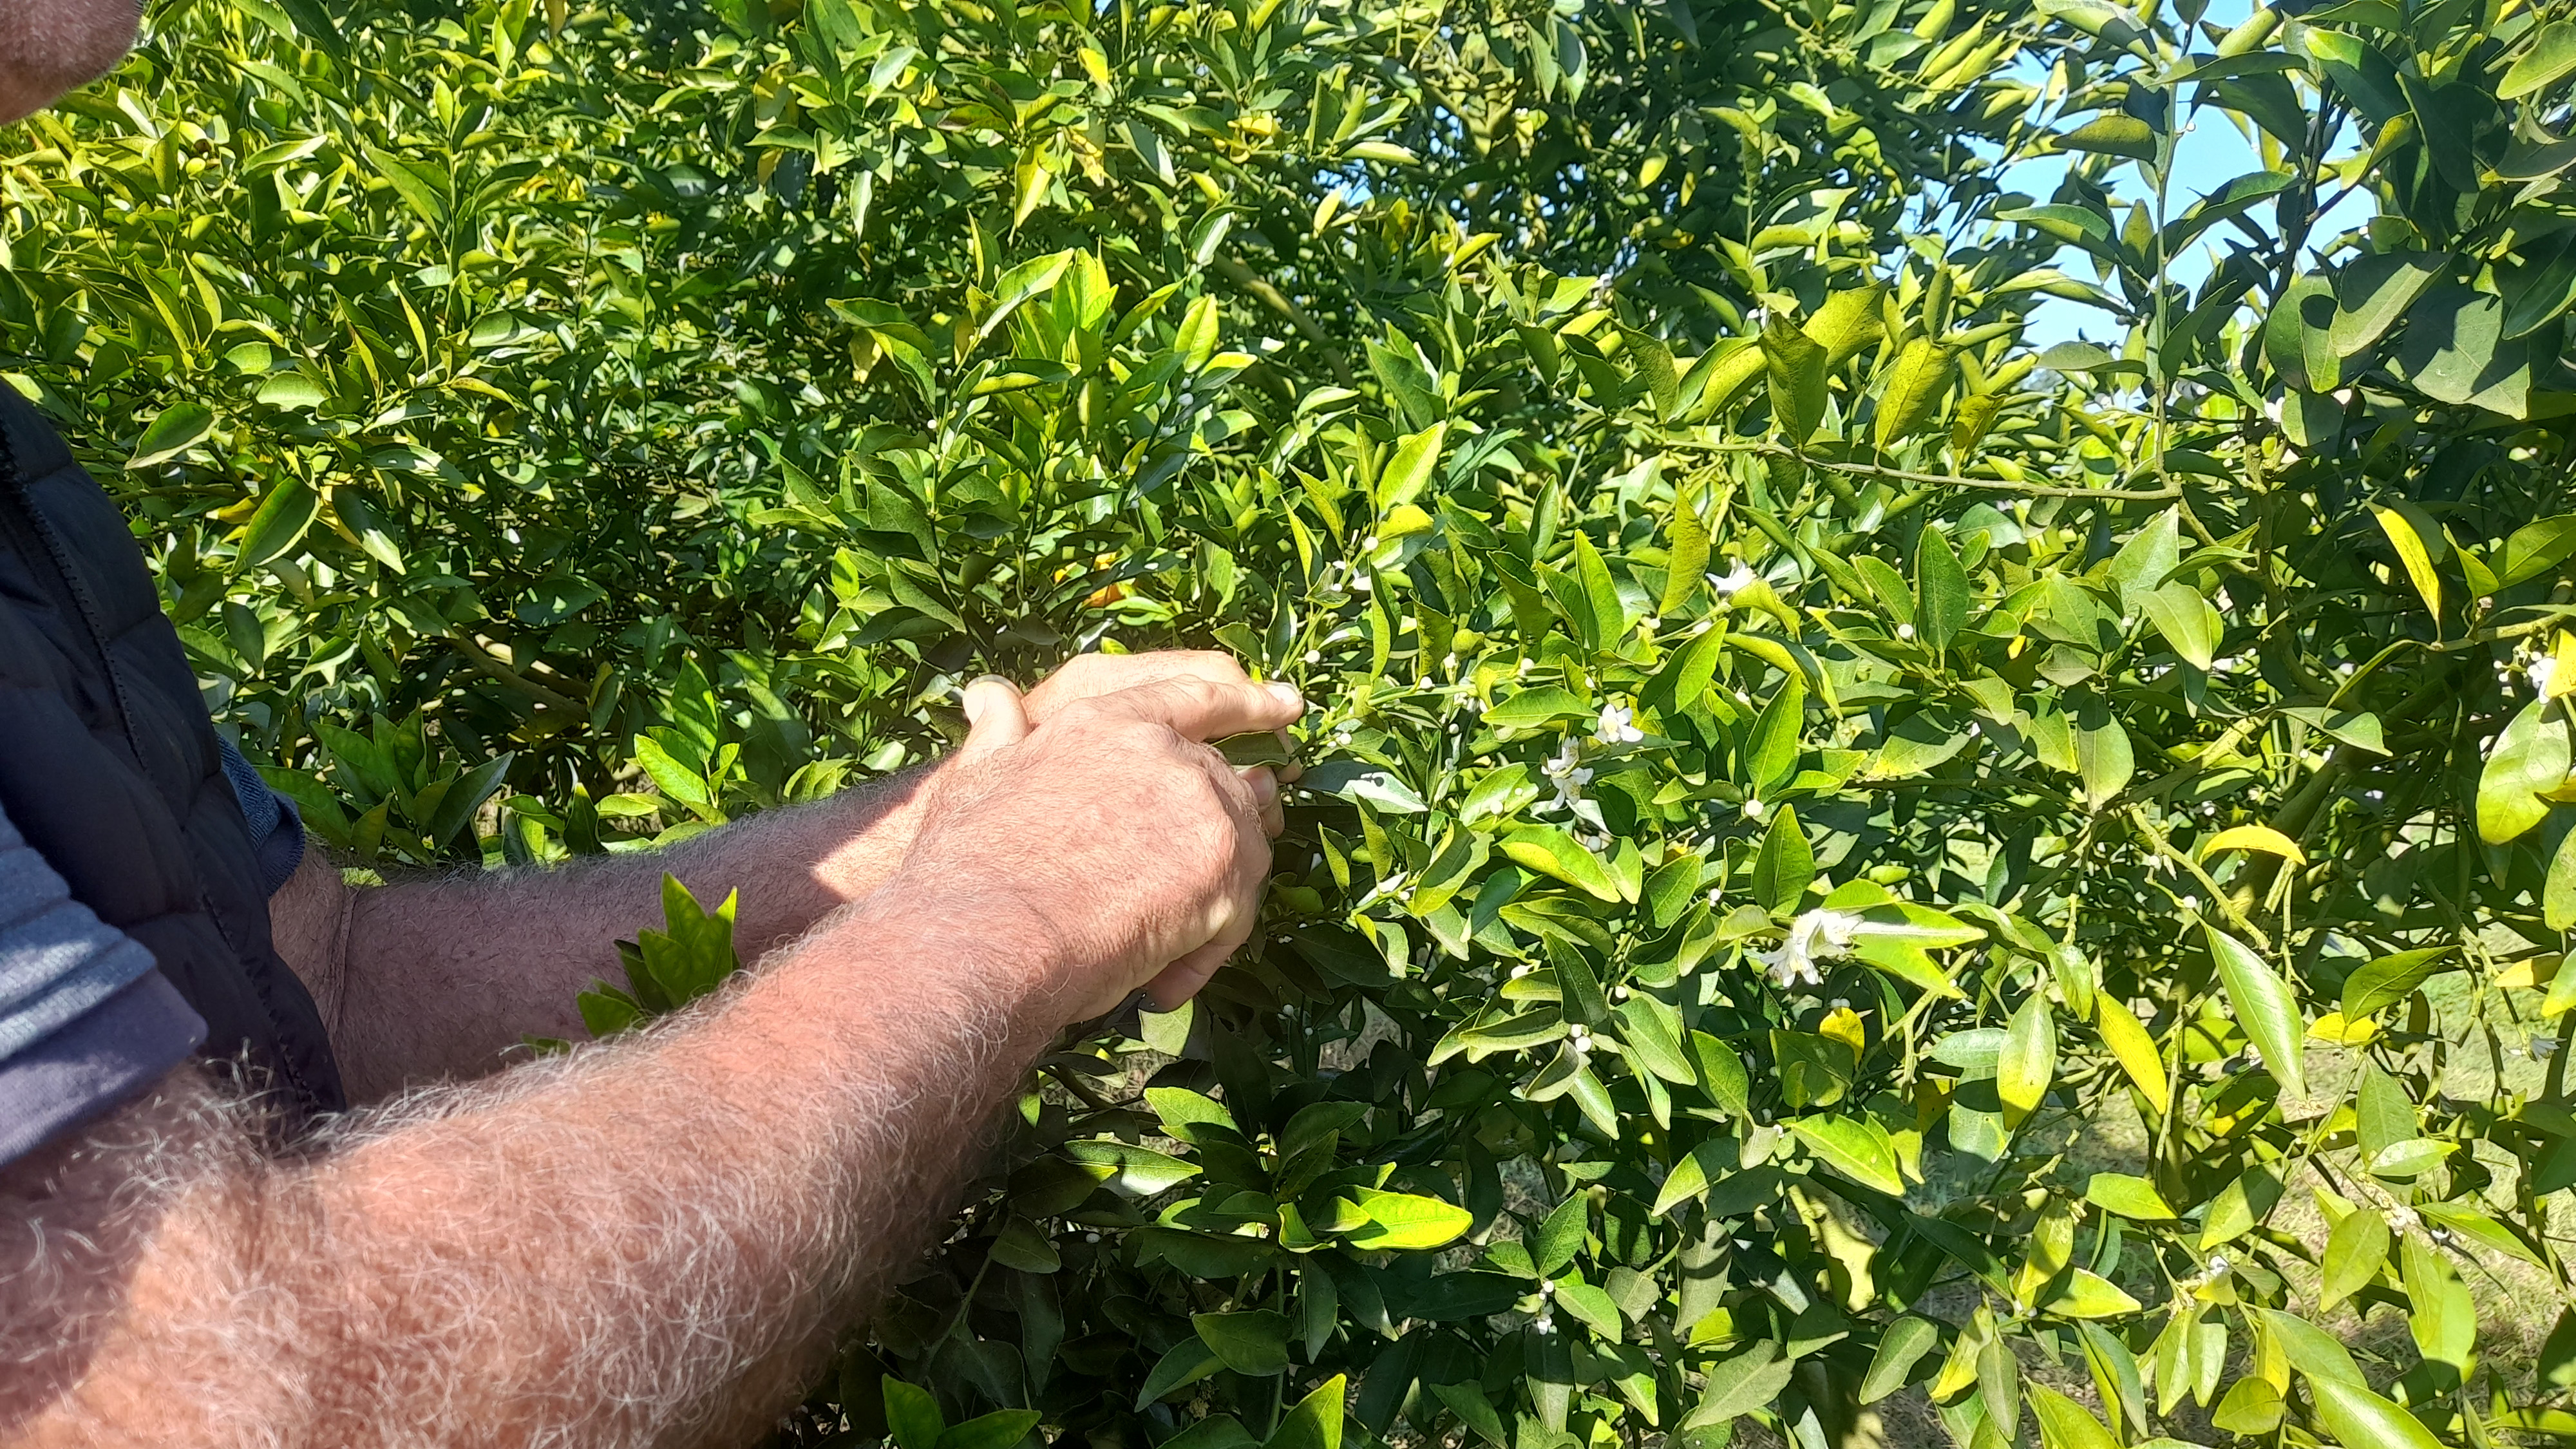
\includegraphics[width=0.8\textwidth]{Images/PesquisaCampo1.jpg}
\SourceOrNote{Equipe 21 - Vitalliz (2025)}
\end{figure}

\medskip
O Entrevistado A relatou que, em sua fazenda, já ocorreram deficiências de 
manganês e cobre nas plantas de \textit{Citrus reticulata} (mexerica). 
A suspeita surgiu devido ao amarelamento das folhas e à clorose internerval. 
A correção dessas deficiências foi realizada por meio da adubação com 
fertilizantes enriquecidos com os nutrientes necessários. O entrevistado 
afirmou conseguir distinguir alguns casos de deficiência de manganês e cobre 
e relatou já ter tido contato com a doença \textit{Greening}, identificada 
por sintomas como amarelamento e presença do \textit{Psilídeo}; nesses casos, 
houve perda total dos frutos. 

\medskip
Em sua fazenda, a falta de nutrientes é frequente, sendo o diagnóstico 
realizado por indicadores como amarelamento das folhas, frutos pequenos e 
produção reduzida. Mais da metade dos casos diagnosticados refere-se a deficiências 
nutricionais gerais. O entrevistado também destacou que um dos principais problemas 
enfrentados é o controle de pragas, e que, quando há algum problema na saúde das 
plantas, busca auxílio de técnico ou agrônomo. Além disso, realiza a verificação 
da saúde das plantas uma vez por mês. Ele e sua equipe contam com o auxílio de aplicativos 
e o apoio de especialistas para a verificação e controle das plantações. 

\begin{figure}[H]
\centering
\caption{Entrevistado A - Sinalização de árvore suspeita }%
\label{fig:Pesquisa-1}
\includegraphics[width=0.8\textwidth]{Images/PesquisaCampo2.jpg}
\SourceOrNote{Equipe 21 - Vitalliz (2025)}
\end{figure}

O Entrevistado A sinaliza árvores suspeitas utilizando uma fita. 
Essas plantas permanecem em observação para tratamento posterior, 
sob acompanhamento do técnico agrônomo.

\medskip
O Entrevistado B relatou ter enfrentado problemas de deficiência de manganês e cobre
em suas plantas, cuja identificação ocorreu por meio do diagnóstico realizado por um engenheiro 
agrônomo, que indicou as medidas corretivas. Em algumas ocasiões, esse profissional também 
realiza análise foliar. O entrevistado afirma conseguir distinguir as deficiências nutricionais 
da doença \textit{Greening} por meio da observação de sintomas, e relata já ter tido 
\textit{Greening} em sua fazenda. O diagnóstico baseia-se na experiência dos funcionários e 
na observação do estado da árvore e dos frutos, porém é tardio, pois as alterações nas folhas 
ocorrem somente em plantas já afetadas. Existem casos em que a planta continua produzindo frutos 
saudáveis mesmo estando doente; nesses casos, o pé não é cortado, apenas tratado, para evitar a 
disseminação da doença para outras plantas. Houve perda parcial da plantação devido ao 
\textit{Greening}, mas havia possibilidade de recuperação. Também são frequentes o amarelamento,
a perda e a diminuição dos frutos na fazenda. 

\medskip
O entrevistado afirma que a maioria dos casos de deficiência nutricional está relacionada
à falta de manganês. Os principais problemas enfrentados no cotidiano da plantação são a 
falta de conhecimento da maioria dos colaboradores para identificar problemas de saúde nas 
plantas de \textit{Citrus reticulata} (mexerica), o que se deve, em parte, ao predomínio do 
cultivo de banana na região, reduzindo o conhecimento específico sobre a cultura cítrica. 
Quando ocorre algum problema na plantação, é chamado um técnico para avaliar e corrigir 
eventuais problemas, como ácaros nos frutos, e as deficiências nutricionais acabam ficando 
em segundo plano. 

\medskip
O entrevistado realiza monitoramento da saúde das plantas em média uma vez por semana, 
geralmente por meio da observação dos funcionários durante o trabalho no pomar. 
Regularmente, não são utilizadas tecnologias para medir a saúde das plantas, mas, 
pontualmente, foram empregados adesivos amarelos para atrair insetos transmissores 
do \textit{Psilídeo}, drones para testar a aplicação de caldas e marcação com fita
plástica para monitorar plantas suspeitas de \textit{Greening}. 

\medskip
Diante das observações realizadas durante a pesquisa de campo, evidencia-se a 
importância deste estudo para a melhoria das práticas de manejo nutricional e 
fitossanitário nas plantações de \textit{Citrus reticulata} (mexerica). 
Verificou-se que o diagnóstico das deficiências nutricionais, especialmente 
de manganês e cobre, ainda ocorre de forma tardia e, em muitos casos, 
é confundido com sintomas da doença \textit{Greening}, resultando 
em perdas significativas na produção e no descarte de plantas potencialmente 
produtivas. O presente projeto propõe o desenvolvimento de um método de 
diagnóstico precoce das deficiências nutricionais por meio da análise foliar 
automatizada, reduzindo a necessidade de acompanhamento técnico constante e 
facilitando o monitoramento direto pelos produtores.
\medskip

% --- Análise Swot ---
\section{Análise Swot}
\medskip
    \label{sect:Analise-Swot}
    A análise SWOT foi realizada com o objetivo de compreender os principais
pontos fortes, fracos, oportunidades e ameaças relacionadas ao projeto NitrusLeaf.

\begin{figure}[H]
\begin{table}[h]
\centering
\caption{Quadro Scrum com tarefas do projeto}
\renewcommand{\arraystretch}{1.2}
\begin{tabularx}{\textwidth}{|>{\raggedright\arraybackslash}X|>{\raggedright\arraybackslash}X|}
\hline
\textbf{Pontos Fortes} & \textbf{Fraquezas} \\
\hline
\begin{itemize}[left=0pt]
  \item É alinhado com iniciativas sustentáveis.
  \item Melhora a eficiência e rapidez no diagnóstico de doenças.
  \item Reduz o risco de pés de mexerica ainda saudáveis.
  \item Reduz o desperdício de alimentos saudáveis.
  \item É alinhado com os objetivos da ODS.
\end{itemize}
&
\begin{itemize}[left=0pt]
  \item Poucos estudos na área envolvendo plantas cítricas.
  \item O treinamento do modelo de IA depende de um grande banco de dados.
  \item O diagnóstico depende da qualidade da imagem.
  \item Dificuldade de acesso à internet por parte dos produtores.
\end{itemize}
\\
\hline
\textbf{Oportunidades} & \textbf{Ameaças} \\
\hline
\begin{itemize}[left=0pt]
  \item Expandir para outras deficiências como: zinco, ferro etc.
  \item Parcerias com empresas, cooperativas e universidades para divulgar o produto.
  \item Crescente demanda por agricultura de precisão.
\end{itemize}
&
\begin{itemize}[left=0pt]
  \item Resistência por parte dos produtores tradicionais.
  \item Concorrência com outras soluções, como drones, por exemplo.
\end{itemize}
\\
\hline
\end{tabularx}
\end{table}
\SourceOrNote{Equipe 21 — Vitalliz (2025).}
\end{figure}
\medskip

Esse tipo de avaliação permite identificar elementos que podem impactar
diretamente o sucesso do sistema, além de apontar caminhos para melhorias contínuas
e decisões estratégicas.

\clearpage
\end{document}